\documentclass[12pt,a4paper]{article}
\usepackage[T1]{fontenc}
\usepackage[utf8]{inputenc}
\usepackage{lmodern}
\usepackage[ngerman]{babel}
\usepackage[numbers]{natbib}
\usepackage{amsmath}
\usepackage{amsfonts}
\usepackage{amssymb}
\usepackage{rotating}
\usepackage{graphicx}
\usepackage[onehalfspacing]{setspace}
\usepackage[left=2.5cm,right=2.5cm,top=2.5cm,bottom=2cm]{geometry}
\usepackage[labelfont=bf]{caption} 
\usepackage{subcaption} %package für gesplittete Grafiken
\usepackage{siunitx} %package für Einheiten\\
\sisetup{separate-uncertainty}
%\usepackage{float}
\usepackage{physics}
%\usepackage{fancyvrb}%package-Erweiterung für verbatim
\usepackage{color}
\usepackage[procnames]{listings}
\usepackage{hyperref} %package für Verlinkungen
\usepackage{multirow} %package für multizeilen in tabellen
%\usepackage{trfsigns}
%\usepackage[labelfont={bf}]{caption} %ermöglicht globale Margins für Captions und andere Einstellungen
\usepackage{floatrow} % package ermöglicht sideways captions
\floatsetup[table]{capposition=top}
\pdfoptionpdfminorversion=6

\clubpenalty=10000   % letzte Zeile einer Seite nicht erste Zeile eines Absatzes
\widowpenalty=10000  % letzte Zeile eines Absatzes nicht erste Zeile einer Seite

\usepackage{upgreek}

\usepackage{textcomp}             % \textperthousand  (promille)
\newcommand{\code}[1]{\texttt{#1}} % Neue Definition für Code im Text
\begin{document}
\bibliographystyle{abbrvdin}
	
\definecolor{keywords}{RGB}{0,51,255}
\definecolor{comments}{RGB}{0,0,113}
\definecolor{red}{RGB}{160,0,0}
\definecolor{green}{RGB}{0,150,0}
\lstset{language=Python, 
	basicstyle=\ttfamily\small, 
	keywordstyle=\color{keywords},
	commentstyle=\color{comments},
	stringstyle=\color{red},
	showstringspaces=false,
	identifierstyle=\color{green},
	procnamekeys={def,class},
	numbers=left}
	\begin{titlepage}
		\begin{center}
			\textbf{\huge Bergische Universität Wuppertal \\[1cm] APP - Gruppe B
			}\\[0.8cm]
			
		\begin{minipage}{0.327\textwidth}
			\centering
			\textbf{\large Dennis Halbach}\\
		    \textbf{\large Henrik Jürgens}\\
		\end{minipage}
		\begin{minipage}{0.327\textwidth}
			\centering
			\textbf{\large Martin Jonas}\\
			\textbf{\large Linus Tischner}\\
			\textbf{\large Philipp Pagel}\\
		\end{minipage}
		\begin{minipage}{0.327\textwidth}
			\centering
			\textbf{\large Philip Bergmann}\\
			\textbf{\large Fabian Heldmann} \\
		\end{minipage}\\[0.5cm]

		\begin{figure}[H]
			\centering
			
\includegraphics[scale=0.3]{uni-logo.pdf}
		\end{figure}

			{ \textbf{\huge Berechnung und Vermessung des Magnetfelds einer Helmholtzspule}}\\[1.5cm]
			\end{center}
		\textbf{Umriss}\\
		In diesem Projekt wird das Magnetfeld eines Helmholtzspulenpaares untersucht. Es wird ein Hallsensor aus drei einzelnen Sonden gefertigt, der das Magnetfeld als vektorielle Größe im Raum bestimmt. Hiermit wird gezeigt, dass ein Spulenpaar in Helmholtzkonfiguration (hier mit Abstand $d=\bar{r}= \SI{15.55(1)}{cm}$) im Inneren einen nahezu homogenen Bereich innerhalb einer Kreisfläche mir Radius $r_H\sim \SI{5}{cm}$. Außerdem werden die Grenzen des verwendeten Messverfahrens aufgezeigt. Es konnte gezeigt werden, dass die Messdaten die theoretischen Erwartungen für das Feld bestätigen und sich Magnetfelder somit gut vorhersagen und berechnen lassen.
			\vfill
		\begin{center}	
			{\large\today}
		\end{center}
	\end{titlepage}
	
	\setcounter{tocdepth}{2}
	\tableofcontents
	\thispagestyle{empty}
	%\listoftables
	\newpage
	
%	\setcounter{secnumdepth}{3} %Befehl für Buchstaben in Kaptielnummerierung in 3.Ordnung
%	\renewcommand*{\thesubsubsection}{\thesubsection.\alph{subsubsection}} 

%\pagestyle{headings}
\section{Motivation und Ziel}
Im Rahmen des Anfänger-Projekt-Praktikums soll Studenten das praktische und selbstständige Arbeiten in Gruppen in der Physik näher gebracht werden. Im Gegensatz zu den anderen Praktika wird hier das Thema des Versuches selbst gewählt. Auch die Planung, der Aufbau, sowie die Durchführung und Auswertung des physikalischen Experiments wird selbstständig von der Arbeitsgruppe durchgeführt. Begleitet und unterstützt wird die Gruppe von Mitarbeitern der Fachgruppe Physik der BUW, die ihr mit Rat und praktischen Vorschlägen zur Seite stehen. Da der Fokus auf den eben beschriebenen Punkten liegt, sollte die Physik größten Teils bekannt sein.\\ 

Magnetfelder stellen als Teil der Elektrodynamik einen weitestgehend verstandenen Bereich der Physik dar. Sie können durch geschickte technische Realisierung der Felder in vielen Bereichen nützlich sein. Beispiele dafür sind magnetische Linsen, Wirbelstrombremsen oder ein Helmholtzspulenpaar als Erzeuger eines annähernd homogenen Magnetfelds. Letztere Eigenschaft wird häufig in physikalischen Praktika genutzt, ohne dass diese analytisch gezeigt wird. Das homogene Magnetfeld kommt durch eine besondere Anordnung von zwei identischen kurzen Spulen zustande. Der Abstand zwischen den beiden Spulen muss genau dem Radius der Spulen entsprechen, damit sich im Raum zwischen den Spulen ein nahezu homogenes Magnetfeld aufbaut. \\ 

Ziel dieses Versuchs ist es, das Magnetfeld eines Helmholtzspulenpaars experimentell zu bestimmen und mit numerisch berechneten Werten zu vergleichen. Hierbei wird kontrolliert, in welchem Bereich der Spule das Magnetfeld als homogen angenommen werden kann. Außerdem wird untersucht, wie stark die Homogenität des inneren Magnetfelds abnimmt, wenn der Spulenabstand verdoppelt wird. Zwecks Messung des Magnetfelds wird ein Hallsensor gebaut, der aufgrund der Nutzung von drei Hallsonden in der Lage ist, das Magnetfeld als vektorielle Größe zu erfassen.


\section{Theorie}
Im Folgenden soll eine Übersicht über die, für die Auswertung des Versuches nötigen, theoretischen Grundlagen gegeben werden.
\subsection{Magnetfeld eines Helmholtzspulenpaars}
Um das Magnetfeld einer Spule zu bestimmen, wird das Biot-Savart Gesetz benutzt, welches direkt aus den Maxwell'schen Gleichungen folgt:
\begin{align}
\textbf{B}(\textbf{r}) = \frac{\mu_0}{4\pi}\int_{V} \dd[3]{r'} \cdot \textbf{j}(\textbf{r}) \times \frac{\textbf{r}-\textbf{r}'}{|\textbf{r}-\textbf{r}'|^3}
\end{align}
Da eine zylindrische Spule verwendet wird, ist es sinnvoll, das Integral in Zylinderkoordinaten darzustellen.
Angenommen wird, dass die Stromdichte in der Spule
\begin{equation*}
|\textbf{j}(\textbf{r})| := \text{j} = \frac{n\cdot\text{I}}{\Delta\text{R}\cdot\text{b}} \text{ mit } \text{R}<r<\text{R}+\Delta\text{R} \text{ und} -\text{b}/2<w<\text{b}/2
\end{equation*} homogen über den Spulenquerschnitt verteilt ist und in Richtung des Einheitsvektors e$_{\varphi}$ zeigt. Dabei ist $\text{R}$ der Innenradius der Spule, $\Delta \text{R}$ ihre Dicke in radialer Richtung und $\text{b}$ ihre Breite. $\text{I}$ ist dabei der Strom, der durch die $n$ Windungen der Spule fließt. Außerhalb der Spule gilt natürlich $\textbf{j} = 0$.
Nach einigen Umformungen erhält man ein Integral, welches das Magnetfeld an einem beliebigen Ort bestimmt:
\begin{align}
\textbf{B}(\textbf{r}) = \frac{\mu_0\cdot\text{j}}{4\pi}\int_{-b/2}^{b/2}\dd w\int_{0}^{2\pi}\dd \phi\int_{R}^{R+\Delta R}\dd r\cdot r \frac{\begin{pmatrix}
	\cos(\phi)\cdot (z-w) \\
	\sin(\phi)\cdot (z-w) \\
	r-(y\sin(\phi)+x\cos(\phi))
	\end{pmatrix}}{\sqrt{(x-r\cos(\phi))^2+(y-r\sin(\phi))^2+(z-w)^2}^3}
\label{eq:Btheo}
\end{align}
\indent Dieses Integral ist im Allgemeinen nicht analytisch lösbar, weshalb es hier durch numerische Integration gelöst wird (vgl. Abschnitt \ref{ch:code}, Code 1). Für die Berechnung des Feldes eines Paars von Spulen, wie es untersucht wird, kann die Formel aufgrund des Superpositionsprinzips im Koordinatensystem gedreht, verschoben und überlagert werden. Der technische Strom fließt bzgl. der z-Achse im mathematisch positiven Sinn, bzw. die Elektronen in der Spule fließen im Uhrzeigersinn. Die Spule liegt dabei in der x-y-Ebene mit dem Schwerpunkt im Ursprung.
\subsection{Erwärmung der Spule bei hohen Strömen}
\label{th:erwärmung}
Um abschätzen zu können, wie viel Strom durch die Spule geschickt werden kann, wird eine Temperaturkurve aufgenommen und mit einer Exponentialfunktion gefittet, um eine obere Schranke für die Temperatur der Spule bei Dauerbetrieb festzustellen. Die Begründung für einen Exponentialfit findet man unter den folgenden Annahmen:
\begin{enumerate}
	\item Das Volumen V der Spule ist auch unter Erwärmung quasi konstant.
	\item Die Raumtemperatur T$_\text{R}$ ist konstant, die Spule befindet sich also in einem konstanten Wärmebad mit "`unendlicher Wärmekapazität"'.
	\item Der Widerstand R der Spule steigt linear mit der Spulentemperatur T. Dies gilt in der Realität für geringe Temperaturänderungen approximativ.
	\item Die Abkühlung der Spule erfolgt nach dem Newton'schen Abkühlunsgesetz.
\end{enumerate}
Die den Prozess beschreibende Differentialgleichung folgt aus den folgenden Überlegungen:\\

\noindent\textbf{Erwärmung der Spule}:\\
Aus der Thermodynamik wird die Formel für die Änderung der inneren Energie E der Spule verwendet und mit der elektrischen Energie, welche von der Spule durch den Strom I absorbiert wird, gleichgesetzt. C ist dabei die Wärmekapazität der Spule.
\begin{align*}
\dd E|_V =& \dd{Q} = \frac{\dd Q}{\dd T^{(1)}}\dd T^{(1)} = \text{C}\cdot\dd T^{(1)}\\
\dd E|_V =& \text{ P}\cdot\dd{t} = \text{R}\cdot\text{I}^2\cdot \dd t
\end{align*}
Daraus folgt für die Erwärmung dT$^{(1)}$ der Spule in Abhängigkeit der Zeit:
\begin{align*}
\dd T^{(1)} = \frac{1}{C}\cdot(a\text{T}+b)\cdot\text{I}^2\cdot \dd t
\end{align*}
wobei $\text{R}:= a\text{T}+b$ nach Voraussetzung eingesetzt wurde.\\

\noindent\textbf{Abkühlung der Spule}:\\
Für die Wärmeemission dT$^{(2)}$ der Spule wird das Newtonsche Abkühlungsgesetz (vgl. \cite{hemmert}) verwendet. K ist eine Proportionalitätskonstante.
\begin{align*}
\dd T^{(2)} = \text{K}(\text{T}-\text{T}_{\text{R}})\dd t
\end{align*}
Die Änderung der Spulentemperatur dT als Summe der Wärmeemission und Absorbtion  hat nun die Form:
\begin{align}
\dd T = \dd T^{(1)}+\dd T^{(2)} = (A\cdot T+B)\dd t
\end{align}
A und B ergeben sich dabei aus den anderen Konstanten.
Dies ist eine lineare inhomogene DGL 1. Ordnung, welche von einer Exponentialfunktion der Form $\text{T}(t)=\text{C}\cdot \exp(\text{A}t)-\text{B}$ gelöst wird.

\subsection{Hallsonden und Hallspannung}
\label{ch:hall}
Befindet sich ein Leiter in einem externen Magnetfeld $\vec{B}$, so werden die Ladungsträger in dem Leiter durch die Lorentzkraft senkrecht zur Bewegungsrichtung und senkrecht zum Magnetfeld abgelenkt. Die so entstehende Ladungstrennung erzeugt ein elektrisches Feld $\vec{E}$, welches der ablenkenden Kraft entgegenwirkt, so dass sich ein Gleichgewicht einstellt. Die dadurch entstandene Potentialdifferenz wird Hallspannung $U_H$ genannt und kann gemessen werden.\\
\begin{figure}
	\centering
	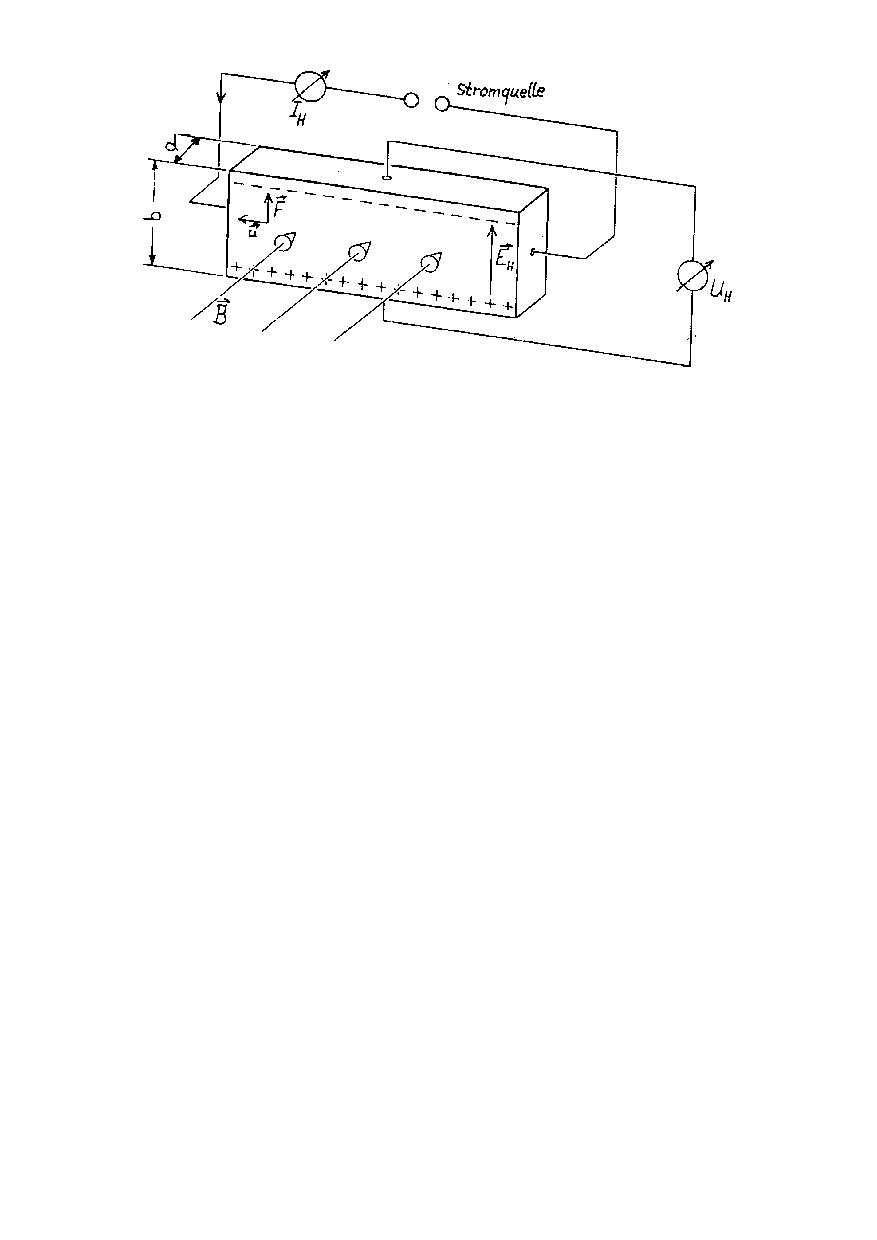
\includegraphics[scale=1]{E2.pdf}
	\caption{Schematische Skizze einer Hallsonde. $\vec{u}$ entspricht der Driftgeschwindigkeit $v_d$. Quelle: \cite{kind}}
	\label{e2}
\end{figure}
Im Gleichgewichtsfall gilt folgende Beziehung: 
\begin{equation}
	e \cdot v_d\cdot B = e \cdot E
	\label{eq:hallGleichgew}
\end{equation}
Dabei sind e die Elementarladung, $v_d$ die Driftgeschwindigkeit der Elektronen, B ist die Komponente des Magnetfeldes senkrecht zum Strom $I_H$ und $E$ ist die elektrische Feldstärke, die durch den Halleffekt erzeugt wird. Das elektrische Feld steht senkrecht auf Strom und Magnetfeld, deshalb kann die Hallsonde das Magnetfeld nur in einer Raumrichtung bestimmen. Diese wird durch die Stromrichtung, der Goemetrie der Hallssonde und den Abgriffpunkten für die Hallspannung festgelegt (vgl. Abb. \ref{e2}).\\
Die Driftgeschwindigkeit $v_d$ kann  wie folgt bestimmt werden:
\begin{equation} 
	v_d = \frac{I_H}{n e\cdot A}
	\label{eq:hallDriftgeschw}
\end{equation}
Hier sind n die Anzahl der Ladungsträger (pro Volumeneinheit) und A ist der Querschnitt des Leiters. Aus den Gleichungen \ref{eq:hallGleichgew} und \ref{eq:hallDriftgeschw}, sowie aus $U=Ed$, ergibt sich:
\begin{equation}
	U_H = \frac{d}{ne\cdot A} \cdot B \cdot I_H
	\label{eq:Hallspannung}
\end{equation}
Dabei ist $d$ die Breite der Sonde; die Distanz, über die sich das elektrische Feld bildet. Außerdem wurde für diese Herleitung angenommen, dass es sich um eine quaderförmige Sonde handelt. Aus der Gleichung \ref{eq:Hallspannung} wird ersichtlich, dass die Hallspannung $U_H$ direktproportional zu der Magnetfeldkomponente B, sowie zum Hallstrom $I_H$ ist. Es ist noch zu erwähnen, dass Hallsonden eine temperaturabhängigkeit in der Hallspannung haben, die vom Sondentyp abhängt. (vgl. Datenblatt Sonde typ KSY 44: \cite{hall})
\section{Versuchsaufbau}
\subsection{Materialliste und Parameter}
Für den Versuch werden die folgenden Materialien verwendet:
\begin{itemize}
	\item Hallsensoren Typ KSY 44 (Datenblatt vgl. \cite{hall})
		\subitem lineare Hallspannung bis $\SI{0.5}{T}$ mit weniger als $0.2\ \%$ Abweichung
		\subitem Temperaturkoeffizient: $\sim -0.03\ \%/\text{K}$
		\subitem Innenwiderstand: (1000 - 1500) $\Omega$
	\item ein Helmholtzspulenpaar mit jeweils
		\subitem Innenradius: \SI{15.0(1)}{\centi m}
		\subitem Außenradius: \SI{16.1(1)}{\centi m}
		\subitem Breite (in Axialer Richtung): \SI{2.0(1)}{\centi m}
		\subitem Windungszahl: $n=130$ (nicht überprüfbare Herstellerangabe)
	\item Koordinatenunterlage mit Millimeterskala
	\item nichtmagnetische Befestigungen (Kupferstäbe, Schraubzwingen, Stativhalterungen sowie zwei optische Bänke mit entsprechenden Reitern)
	\item Leybold Steckbrett
\end{itemize}
Für die Messungen wurden die folgenden externen (Mess-)Geräte verwendet:
\begin{itemize}
	\item Leybold Cassy-System
	\item mehrere Digitalmultimeter
	\item Winkelmesser und Lineale
	\item Konstantstromquellen für geringe ($\sim \SI{7}{mA})$ und hohe ($\sim \SI{4}{A}$) Ströme
\end{itemize}
\subsection{Aufbau}
Der Versuchsaufbau besteht im Kern aus zwei Helmholtz-Spulen, die parallel zueinander aufgestellt sind - zunächst im Abstand des Radius, anschließend im doppelten Abstand, um die Auswirkung des Abstandes auf die Homogenität des Magnetfeldes innerhalb der Spulen zu überprüfen. Damit die Spulen ein gleich starkes Magnetfeld in dieselbe Richtung erzeugen, werden sie bezüglich des Stromes gleichsinnig und in Reihe geschaltet. Alle benötigten Befestigungen sind nach Möglichkeit nicht (ferro-)magnetisch, sodass ein dadurch bedingter systematischer Fehler vermieden wird.\\

Für eine möglichst exakte Messung des Magnetfeldes bieten sich zur Positionierung der Sonde folgende Möglichkeiten an:\\

\noindent \textbf{Koordinatenunterlage}\\
Die Bestimmung der Position der Sonde mithilfe der Koordinatenunterlage ist aufgrund des Abstandes der Sonde zur Unterlage und der Vielzahl an Messpunkten mit großem Zeitaufwand verbunden. Des Weiteren sind die Spulen auf einer Holzplatte befestigt, unter der sich die Koordinaten-Unterlage befindet, was eine präzise Messung für die Messpunkte innerhalb der Spulen, die wie erwähnt von besonderem Interesse sind, unmöglich macht. Die Bestimmung der Position würde also auf die Verwendung eines Lineals zurückfallen, was zu langsam und ungenau ist.\\
\textbf{Ortung mittels Schall}\\
Schallortung wäre prinzipiell eine Möglichkeit der Positionsbestimmung. Die Größe des Piezo-Kristalls stellt allerdings eine immanente Fehlerquelle dieser Messung dar, die – unabhängig von der Genauigkeit der Positionierungsmethode an sich – zu einem Fehler von über einem Zentimeter führt.\footnote{In der Auswertung wird deutlich, warum die Genauigkeit der Position entscheidend ist.} Zuletzt erscheint dieses Vorgehen zeitlich nicht durchführbar.\\
\textbf{Positionsbestimmung mittels sichtbarem Laser}\\
Das Positionieren durch Laser bietet dagegen folgende entscheidende Vorteile: Die Genauigkeit ist größtenteils abhängig von der Dicke des Laserstrahls, die mit ~ 2 mm eine möglichst genaue Messung ermöglicht (vgl. 5.2.1 Unsicherheit in der Positionsbestimmung). Außerdem wird im Gegensatz zur Schall-Ortung keine Zeit für das Entwickeln einer Positionierungsmethode aufgewendet. Der Fokus des Versuchs soll auf der Messung des Magnetfeldes liegen. Wichtig ist zuletzt insbesondere, dass das Verschieben der Sonde durch die Laser so möglichst wenig Zeit in Anspruch nimmt. Dies ermöglicht es offensichtlich, im selben Messzeitraum eine größere Anzahl an Messpunkten aufzunehmen und so eine möglichst ausführliche Auswertung des Spulenmagnetfeldes vornehmen zu können.\\

Die Positionierung geschieht nach folgendem Prinzip: Die Spulen sind von optischen Bänken (die durch eine Koordinatenunterlage millimetergenau ausgerichtet sind) umschlossen, auf denen sich an Stangen befestigt die Laser befinden. Die Laserstrahlen stehen senkrecht zu ihrer jeweiligen optischen Bank und – da sich die Laser auf derselben Höhe befinden – kreuzen sich an einem Punkt über der Koordinatenunterlage. Dies wird ausgenutzt, um die Sonde exakt an diesem Punkt auszurichten.\\
 
Zuerst wird sichergestellt, dass beim Verschieben der Laser in der Höhe diese nicht verdreht wurden. Dies wird durch die Koordinatenunterlage erreicht, auf die ein Winkelmesser gestellt wird. So kann gemessen werden, ob der Laser tatsächlich senkrecht zur optischen Bank strahlt und zudem ob sich die Höhe des Strahls über der Unterlage nicht verändert. Anschließend wird die Stange, an der die Halterung für die Sonden befestigt ist, gedreht, so dass Letztgenannte nicht mehr parallel zu den Spulen ausgerichtet ist. Die Stange wird nun so weit verschoben, bis der Laser, der entlang der x-Achse zeigt (s. Abb. 5), eine Markierung an der Stativhalterung an der Stange trifft. Dreht man die Stange, bis der Laser halb die Stativhalterung und halb die Kante trifft, an der die Hall-Sensoren befestigt sind, ist die Halterung exakt parallel zur x-Achse ausgerichtet. Durch geschicktes Verschieben der Stange ist es möglich, dass nach dem Ausrichten an der x-Achse der zweite Laser ebenfalls halb die Kante der Halterung trifft, sodass die Sensoren perfekt durch die beiden senkrecht aufeinander stehenden Laserstrahlen ausgerichtet sind (vgl. Abb. \ref{ph:1}). Zur graphischen Veranschaulichung dieses Prozesses wird der Versuchsaufbau in Abbildung \ref{fig:sk1} verdeutlicht.\\

Die Stromversorgung der Hall-Sensoren erfolgt, genauso wie bei den beiden Spulen, durch eine Reihenschaltung, um mögliche Fehlerquellen zu minimieren. Dass die Ströme sowohl durch den Sensor als auch durch die Spule konstant bleiben ist hierbei essentiell, da die Hallspannung (vgl. Formel \ref{eq:Hallspannung}) und auch das Magnetfeld der Spule (vgl. Formel \ref{eq:Btheo}) linear von der entsprechenden Stromstärke abhängen. Die Verschaltung der Sensoren ist in Abbildung \ref{sch-sond} skizziert. Die Sensoren werden allerdings, anders als dort dargestellt, aufgrund der begrenzten Anzahl an Anschlüssen des vorhandenen Cassy-Systems nacheinander gemessen. Um dabei nicht die Halterung der Sensoren zu berühren, werden die von den Sensoren wegführenden Drähte für die Hallspannung zu einem Leybold-Steckbrett geführt, so dass die Spannungsanschlüsse unkompliziert und schnell umgesteckt werden können. Der Hallsensor wird gebaut, indem die drei einzelnen Sonden orthogonal zueinander auf das Plexiglas-Trägermaterial geklebt werden (vgl. Abb. \ref{sond-foto}).
Die Sonde misst nun die Hallspannung, welche durch die senkrecht auf ihr stehende Magnetfeldkomponente in den Hallsonden erzeugt wird. Diese wird über das Cassy-System ausgegeben und später in das Magnetfeld umgerechnet (vgl. 4.2.2 Bestimmung des Proportionalitätsfaktors zwischen B und $U_H$ und Berechnung des Magnetfeldes aus der Hallspannung).

\section{Vorversuche}
Im Folgenden wird auf vorbereitende Versuche eingegangen, die wichtige Erkenntnisse und Größen für die eigentliche Messung der Spulenfelder liefern.
\subsection{Abschätzung der Temperaturentwicklung der Spulen}
Wie in Abschnitt \ref{th:erwärmung} gezeigt wurde, stellt sich eine in einem Wärmebad  mit unendlicher Wärmekapazität gelagerte Spule auf eine konstante Temperatur ein, wenn sie von einem konstanten Strom durchflossen wird. Für eine solche Messung kann deshalb eine exponentielle Anpassung gewählt werden. Unser Laborraum erfüllt diese Bedingungen in guter Näherung. Da der Hersteller der Spulen einen maximalen (kurzzeitigen) Strom von \SI{2}{A} empfiehlt (vgl. \cite{leybold}), ist es nötig herauszufinden, ob ein höherer Strom eine kritische Temperatur verursacht. Dies ist in Abbildung \ref{fig:tempcurve} zu sehen.
\begin{figure}[H]
	\centering
	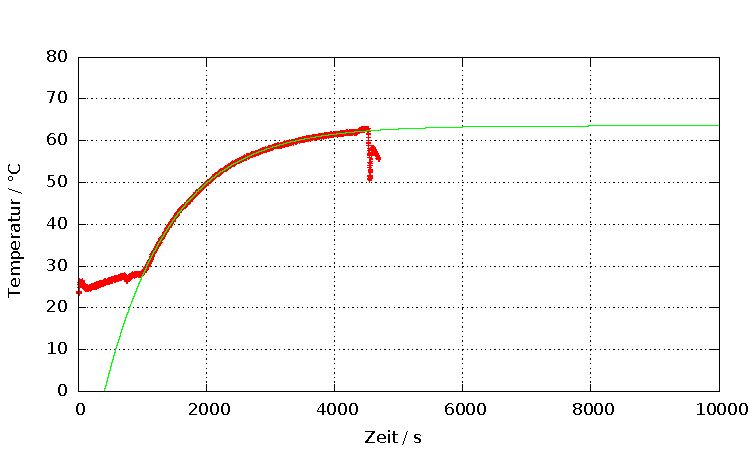
\includegraphics[scale=1]{Temperaturcurve.pdf}
	\caption{Temperatur einer Spule in Abhängigkeit der Zeit bei einer Stromstärke von \SI{4.15}{A}. Zu Anfang fließt ein geringerer Strom. Am Ende der Messreihe sieht man das Abschalten des Stroms und die daraus resultierende schnelle Abkühlung der Spule. Die Raumtemperatur während der Erfassung der Daten betrug \SI{24\pm 1}{\celsius}.}
	\label{fig:tempcurve}
\end{figure}
Man sieht, dass die Temperatur der Spulen eine maximale Temperatur von $T_{max}\simeq \SI{64}{\celsius}$ nicht überschreiten wird. Dieses Ergebnis legt nahe, dass die Verwendung der Spulen bei \SI{4}{A} unbedenklich ist, da die an der Spule befindlichen Materialien erst bei wesentlich höheren Temperaturen ihre Form verändern (z.B. schmelzen). 
\subsection{Kalibration der Sensoren und Erdmagnetfeld}
Die verwendeten Hallsonden des Typs KSY 44 liefern - wie in Abschnitt \ref{ch:hall} gezeigt wurde - eine zum vorliegenden Magnetfeld proportionale Hallspannung. Der tatsächliche Wert des Feldes ist dabei nur bekannt, wenn man den Proportionalitätsfaktor zwischen Hallspannung und Magnetfeld kennt. Dieser soll im Folgenden bestimmt werden.
\subsubsection{Erdmagnetfeld}
Da das Erdmagnetfeld mit etwa \SI{50}{\micro T} einen Beitrag liefert, der zwar klein, aber messbar ist, muss das Magnetfeld aus den Messdaten herausgerechnet werden. Dies wird berücksichtigt, indem vor jeder Messung die Offsetspannung\footnote{Die Offsetspannung ist für jeden Sensor unterschiedlich und wird durch das Erdmagnetfeld beeinflusst.} des Sensors bestimmt und als "`Null"' definiert wird. Da das Erdmagnetfeld innerhalb des Laborraumes so gut wie konstant ist, wird somit die Anwesenheit desselben durch diese Wahl der Nullspannung kompensiert. Somit hat das Erdmagnetfeld keinen Einfluss mehr auf die Messungen. Es muss anschließend darauf geachtet werden, dass der Sensor ausschließlich parallel verschoben wird, da sich ansonsten der Einfluss der äußeren Magnetfelder auf den Hallsensor verändert.
\subsubsection{Bestimmung des Proportionalitätsfaktors zwischen $B$ und $U_H$ und Berechnung des Magnetfeldes aus der Hallspannung CASSY UNGENAU}
Die drei Hallsensoren werden mithilfe eines geeichten Hallsensors kalibriert, der Teil des CASSY-Systems ist (im Folgenden als Eichsensor/Eichsonde bezeichnet). Dazu werden die zu kalibrierende Hallsonde und die Eichsonde so ausgerichtet, dass das vorliegende Magnetfeld senkrecht zu ihnen steht. Dabei steht die Eichsonde ebenfalls senkrecht zum Trägermaterial des zu kalibrierenden Sensors. Dabei muss die Inklination der Sonde gegen das Trägermaterial ignoriert werden, damit die Korrektur in Abschnitt \ref{ch:korr} Gültigkeit besitzt. Zudem ist die Kalibration des Sensors dann (für die entsprechende Komponente) auch ohne Korrektur korrekt. (vgl. Abb. \ref{fig:kalib}, Foto des Setups: Abb. \ref{kalib1}). Der Einfluss der anderen Komponenten muss dann durch die Korrektur berücksichtigt werden. Die Ausrichtung der Sensoren zueinander geschieht mittels der Laser, die später zum Positionieren der Sonde im Magnetfeld verwendet werden (vgl. Abschnitt \ref{sec:versuchsdurchfuhrung}). Die Magnetfeldrichtung wird insofern als bekannt vorausgesetzt, als dass aus Symmetriegründen der Aufbau in Abb. \ref{fig:sk1} in der Mitte der Spule ein Magnetfeld in y-Richtung erzeugt. Zu verschiedenen Magnetfeldstärken wird die Hallspannung $U_H$ der Hallsonde und die gemessene magnetische Flussdichte der Eichsonde bestimmt. Die Unsicherheit der gemessenen Spannungen ist dabei durch die Messbarkeitsgrenze des Cassy-Systems mit $\Delta U = \SI{0.01}{mV}$ gegeben. Die Hallsonde des Cassy-Systems weist starke Schwankungen auf und liefert das Magnetfeld für die Kalibration mit einer Ungenauigkeit der Größenordnung $\SI{0.05}{mT}$.\\

Der daraus entstehende lineare Zusammenhang von Hallspannung zu magnetischer Flussdichte wird für die Bestimmung des Magnetfeldes des Helmholtzspulenpaares verwendet. Die Auswertung der Messung für die Kalibrierung ist in den Abbildungen \ref{kalib_plot_a} bis \ref{kalib_plot_c} zu sehen. Für die Kalibration der Sensoren folgt also:
\begin{table}[H]
	\centering
	\begin{tabular}{c|c|c}
	Sensor\# / Richtung	& $P\stackrel{.}{=}\frac{\Delta B}{\Delta U_H}$[$\frac{\text{T}}{\text{V}}$]  & $\Delta P$ [$\frac{\text{T}}{\text{V}}$] \\ \hline \hline
	1 / z	& $ -0.687$ & 0.01 \\ 
	2 / y	& $ -0.714$ &  0.01\\ 
	3 / x	& $ -0.698$ &  0.01\\ 
	\end{tabular} 
	\caption{Kalibrationsergebnis. Die Vorzeichen ergeben sich dabei aus der Messrichtung der Sensoren und aus der Wahl des Koordinatensystems (vgl. Abb. \ref{fig:sk1}).}
\end{table}
\begin{figure}
	\centering
	\begin{subfigure}[c]{0.7\textwidth}
		\centering
		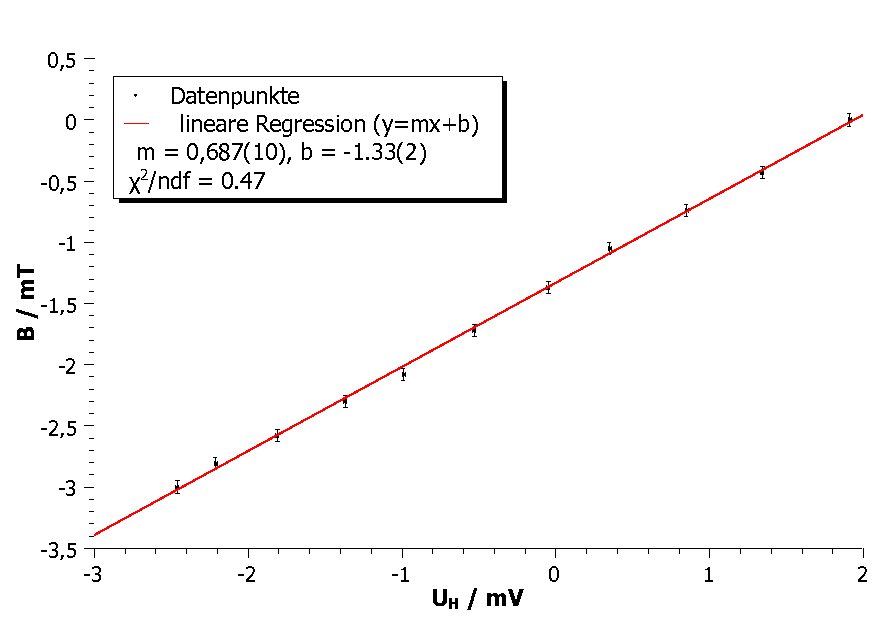
\includegraphics[scale=0.7]{sensor1.pdf}
		\caption{Kalibration von Sensor 1 (z-Richtung).}
		\label{kalib_plot_a}
	\end{subfigure}\\
	\begin{subfigure}[c]{0.7\textwidth}
		\centering
		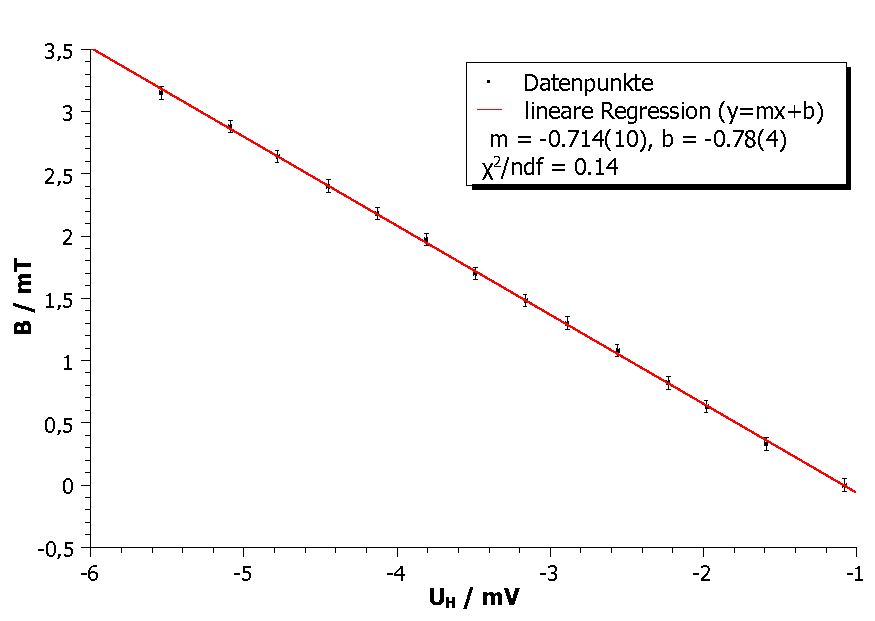
\includegraphics[scale=0.7]{sensor2.pdf}
		\caption{Kalibration von Sensor 2 (y-Richtung).}
		\label{kalib_plot_b}
	\end{subfigure}\\
	\begin{subfigure}[c]{0.7\textwidth}
		\centering
		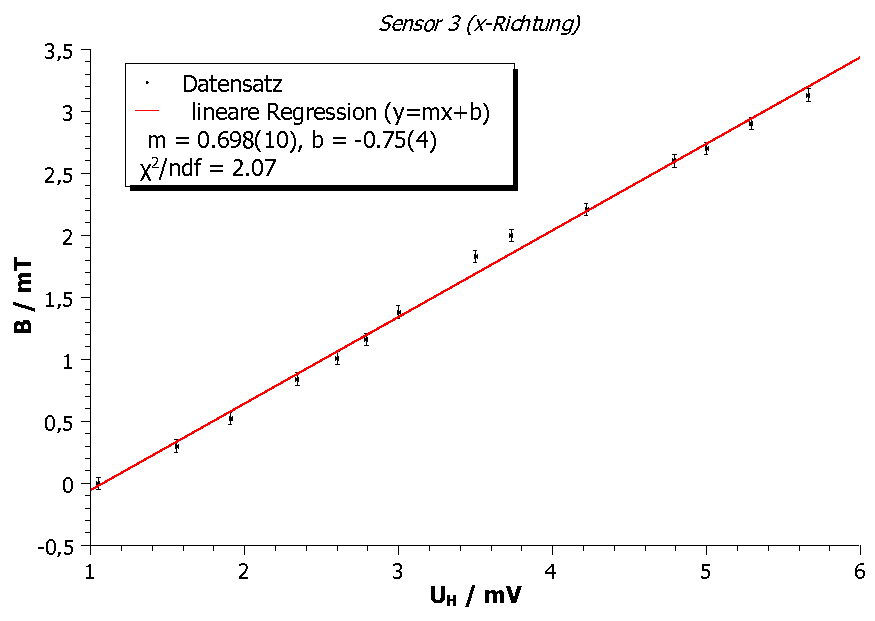
\includegraphics[scale=0.7]{sensor3.pdf}
		\caption{Kalibration von Sensor 3 (x-Richtung).}
		\label{kalib_plot_c}
	\end{subfigure}
	\caption{Auswertung der Kalibrationsdaten}
	\label{fig:kalib_plot}
\end{figure}
Während der Kalibration herrschte eine Raumtemperatur von $\SI{25(1)}{\celsius}$. Sei nun i die Nummer des Sensors, $U_{0,i}$ der Offset der Hallspannung, und $P_i$ der Proportionalitätsfaktor zwischen $U_H$ und $B$. Dann bestimmt sich die Komponente in Richtung von Sensor i des Magnetfelds am Ort \textbf{x} zu
\begin{equation}
	B_i(\textbf{x})=(U_i(\textbf{x})-U_{0,i})\cdot P_i
	\label{eq:B}
\end{equation}
mit dem Fehler
\begin{align}
	\nonumber \Delta B_i(\textbf{x}) &= \sqrt{(\Delta U_i \cdot P_i)^2+(\Delta U_{0,i}\cdot P_i)^2+((U_i-U_{0, i})\cdot \Delta P_i)^2}\\
	 &= \sqrt{2\cdot (\Delta U_i \cdot P_i)^2+((U_i-U_{0, i})\cdot \Delta P_i)^2}
\end{align}
\subsubsection{Konzept einer Korrektur der Kalibrierung}
\label{ch:korr}
Der auf das Trägermaterial geklebte Hallsensor wurde kalibriert, indem jede der Komponenten während der Kalibrierung in Richtung des B-Feldes der Spulen gehalten wurde.
Dafür wurde die Plexiglashalterung mit den Lasern wie bei den Messungen in Richtung des B-Feldes ausgerichtet (siehe \ref{sec:versuchsdurchfuhrung}). Eine mögliche Fehlerquelle bei dieser Kalibrierungsvariante ist die Winkeldifferenz zwischen der Plexiglashalterung und den Hallsonden, da diese mit Heißkleber angeklebt wurden. Experimentell kann man den Winkel einer Sonde zu der Ebene, in der sie eigentlich liegen sollte nur bestimmen, in dem man den Winkel der Hallsonde zu den beiden Achsen dieser Ebene ausmisst.
Betrachtet wird im Folgenden ein rechtshändiges Koordinatensystem bezüglich einer orthonormalen Basis, dessen Achsen als x-,y- und z-Achse  bezeichnet werden. O.B.d.A sei die Ebene, in der die Hallsonde eigentlich liegen sollte, die xy-Ebene. Der Winkel der Hallsondenebene zur x-Achse sei $\alpha$, und der Winkel zur y-Achse sei $\beta$. Für den Winkel $\gamma$ der Ebene der Hallsonde zur xy-Ebene ergibt sich aus $\alpha$ und $\beta$ :
\begin{align*}
\gamma = cos^{-1}\left(\frac{1}{\sqrt{sin^2(\alpha)+sin^2(\beta)+1}}\right)
\end{align*}
Wie im Abschnitt zuvor dargelegt, wurde jede der Sonden nach dem folgenden Prinzip kalibriert: Die Inklination der einzelnen Sonde wird zunächst vernachlässigt, und das äußere Magnetfeld senkrecht zur idealen Sensorposition angebracht, sodass nicht das Magnetfeld, sondern nur die Komponente parallel zur idealen (=gewollten) Richtung gemessen wird. Das heißt aber, dieser Sensor wird in Richtung der eigenen Normalen ein um einen Faktor $\frac{1}{cos(\gamma)}$ größeres B-Feld messen. Dies ist in der folgenden Abbildung anschaulich dargestellt:
\begin{figure}[H]
	\centering
	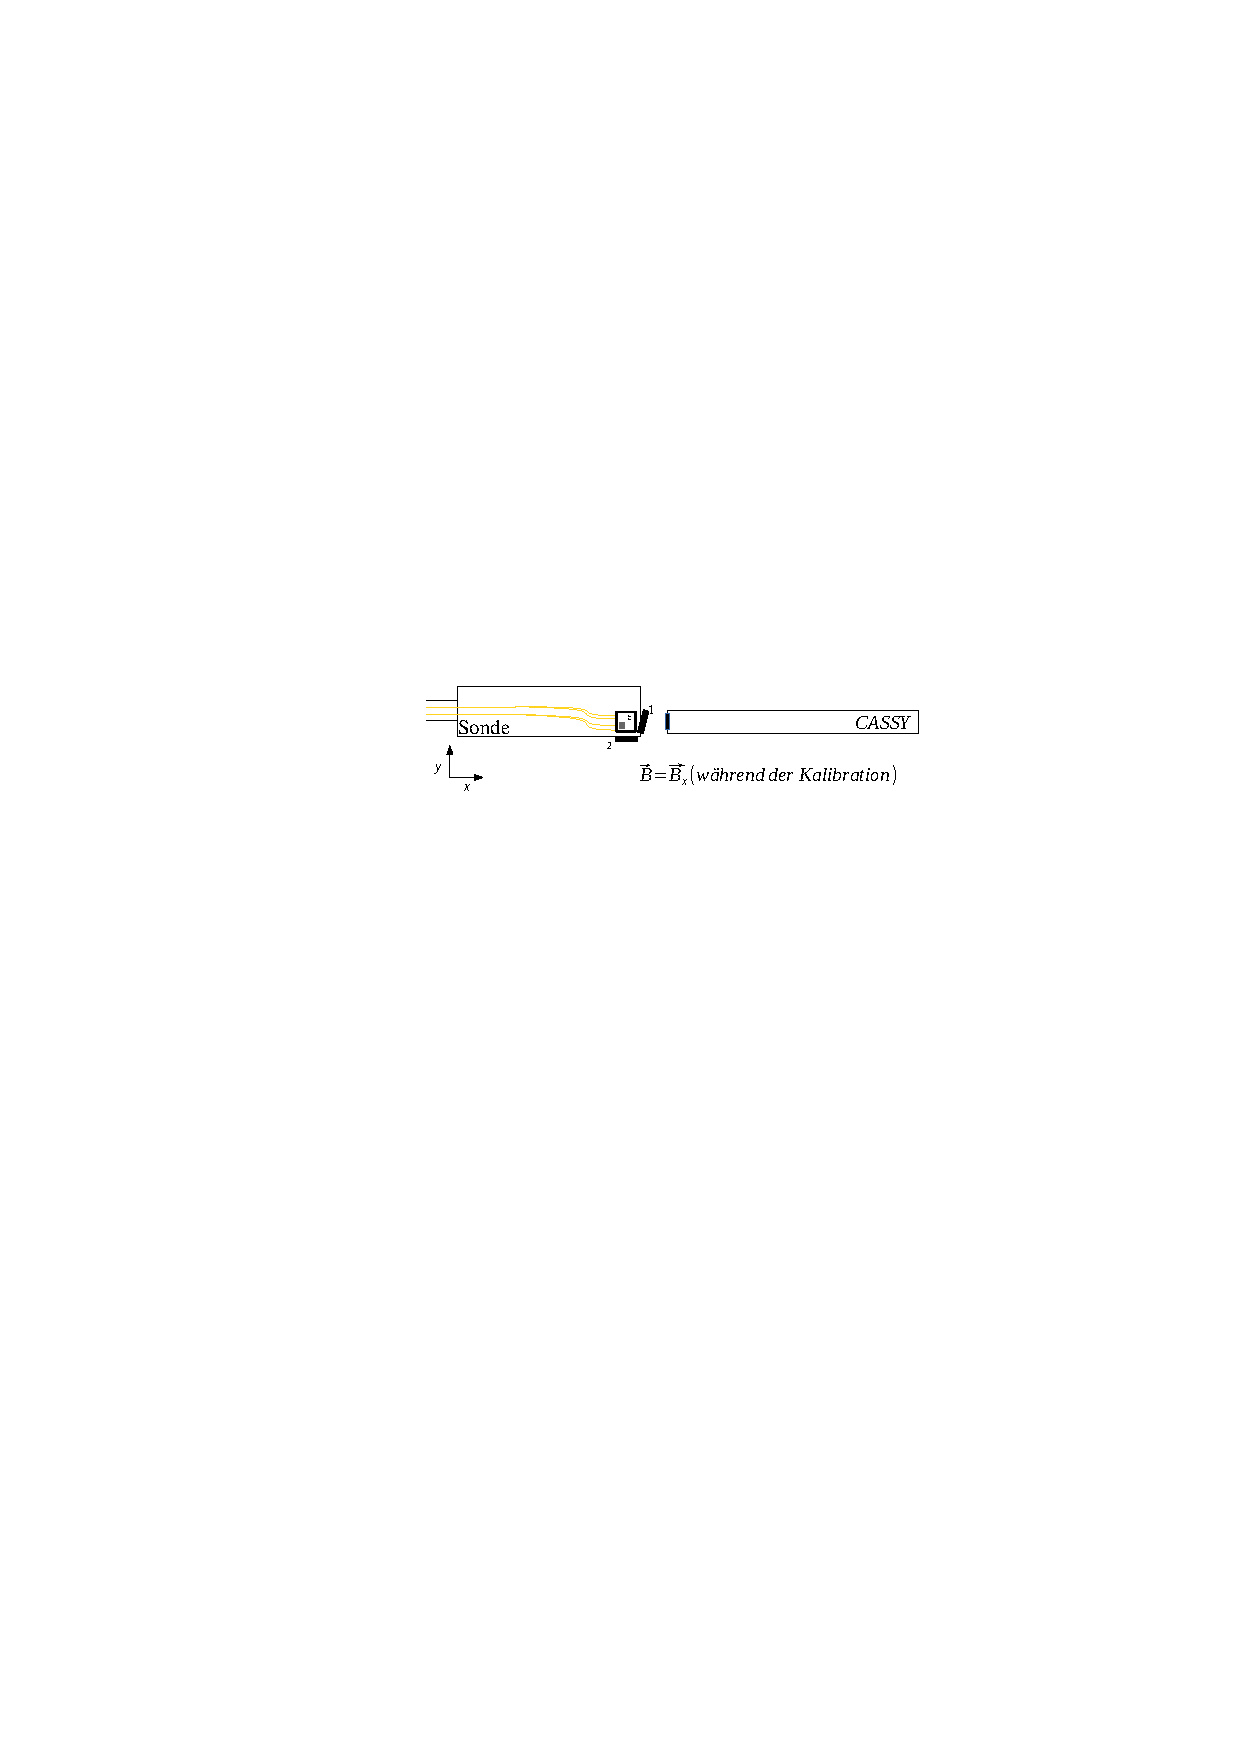
\includegraphics[scale=1.3]{kalib_skizze1.pdf}
	\caption{Zweidimensionale Darstellung des Kalibrationsprozesses. Das Magnetfeld zeigt während der Kalibration nur in x-Richtung. Dies wird durch entsprechende Positionierung des Sensors in der Mitte des Helmholtzspulenpaars erreicht.}
	\label{fig:kalib}
\end{figure}
Das gleiche gilt für die anderen beiden Sensoren. Man kann nun aus diesen zwei Winkeln pro Hallsonde, solange die drei Normalen der Hallsondenebenen linear unabhängig bleiben, das eigentliche B-Feld in Richtung der Koordinatenachsen angeben. Man findet nach geometrischen Überlegungen jeweils einen Ausdruck für die Komponenten $B_x$, $B_y$ und $B_z$ in Abhängigkeit der Winkel, welche noch von den anderen B-Feld-Komponenten abhängen.
\begin{align*}
B_z = B_1-\frac{sin(\alpha_1)B_x+sin(\beta_1)B_y}{cos(\gamma_1)}
\end{align*}
Dabei steht der Index 1 für den dritten Hallsensor, dessen Normale die größte z-Komponente hat.\footnote{Index 3 bzw. 2 steht für den Hallsensor mit größter x- bzw. y-Komponente.} Analoge Ausdrücke folgen für die anderen beiden Komponenten. Dieses lineare Gleichungssystem besteht aus drei Unbekannten und drei unabhängigen Beziehungen. Es kann z.B. mit dem Gauß-Algorithmus oder der Cramerschen Regel gelöst werden. Für unsere Korrektur werden Terme der Form $sin(a)\cdot sin(b)$ vernachlässigt, da in unserem experimentellen Aufbau alle Winkel kleiner als \SI{3}{\degree} sind (Kleinwinkelnäherung). So folgt:
\begin{align}
\label{eq:incl}
\nonumber B_x &\simeq \left( B_3 - \frac{sin(\beta_3)}{cos(\gamma_3)}B_1 - \frac{sin(\alpha_3)}{cos(\gamma_3)}B_2 \right) \cdot \frac{1}{A} \simeq  B_3 - \frac{sin(\beta_3)}{cos(\gamma_3)}B_1 - \frac{sin(\alpha_3)}{cos(\gamma_3)}B_2\\
B_y &\simeq \left( B_2 - \frac{sin(\beta_2)}{cos(\gamma_2)}B_3 - \frac{sin(\alpha_2)}{cos(\gamma_2)}B_1 \right) \cdot \frac{1}{A}\simeq  B_2 - \frac{sin(\beta_2)}{cos(\gamma_2)}B_3  - \frac{sin(\alpha_2)}{cos(\gamma_2)}B_1\\
\nonumber B_z &\simeq \left( B_1 - \frac{sin(\beta_1)}{cos(\gamma_1)}B_2 - \frac{sin(\alpha_1)}{cos(\gamma_1)}B_3 \right) \cdot \frac{1}{A}\simeq  B_1 - \frac{sin(\beta_1)}{cos(\gamma_1)}B_2 - \frac{sin(\alpha_1)}{cos(\gamma_1)}B_3
\end{align}
Dabei ist $A\simeq 1$ (vgl. Abschnitt \ref{eq_formeln} Formel \ref{eq:e1}).\\

\noindent Im Fall unseres realen Aufbaus gelten die folgenden Voraussetzungen in guter Näherung:
\begin{itemize}
	\item Die Hallsensoren in x und z -Richtung haben nahezu keine Inklination in Richtung y, weshalb sie keine Störung durch die y-Komponente des Magnetfeldes erfahren.
	\item Die y-Komponente des Magnetfelds der Spulen ist während den quantitativ relevanten Messungen \textit{deutlich} größer als die x und z Komponente, weshalb die Korrektur der y-Komponente nach Formel \ref{eq:incl} weniger als 1\% des Messwerts in y-Richtung beträgt.
\end{itemize}
Da es an dieser Stelle nicht möglich ist, die Winkel zwischen den Sensoren genau zu bestimmen, und die Korrektur durch die obigen Voraussetzungen ohnehin extrem klein ist, wird sie in der Auswertung der Ergebnisse vernachlässigt.
\subsection{Verstärkung der Hallspannung}
Da das Magnetfeld des Helmholtzspulenpaars auch bei Strömen im Bereich von \SI{4}{A} nur Magnetfelder der Größenordnung einiger Millitesla produziert, beträgt die Ausgangsspannung der Hallsonden nur einige Millivolt. Dies führt zu dem Problem, dass die Spannung über Digitalmultimeter nicht mehr hinreichend genau bestimmt werden kann, da diese höchstens \SI{0.1}{\milli V} Auflösung bieten. Um die Spannung mit Digitalmultimetern genauer messen zu können, ist es nötig, diese zu verstärken. Hierfür kann ein Operationsverstärker verwendet werden.\\

Da die Hallsonden über eine Reihenschaltung mit dem Hallstrom versorgt werden, liegt das absolute Potential an den Ausgängen für die Hallspannung unter Umständen bei bis zu \SI{15}{V} (vgl. Abb.  \ref{sch-sond}). Die obere Grenze des Operationsverstärkers (Typ TL081) ist allerdings durch die Versorgungsspannung mit $\sim\SI{12}{V}$ gegeben, sodass die Hallspannung vor der Verstärkung verkleinert werden muss. Dies wird über einen simplen Spannungsteiler realisiert. Die Schaltung ist in Abbildung \ref{fig:schaltung} zu sehen.
\begin{figure}[H]
	\centering
	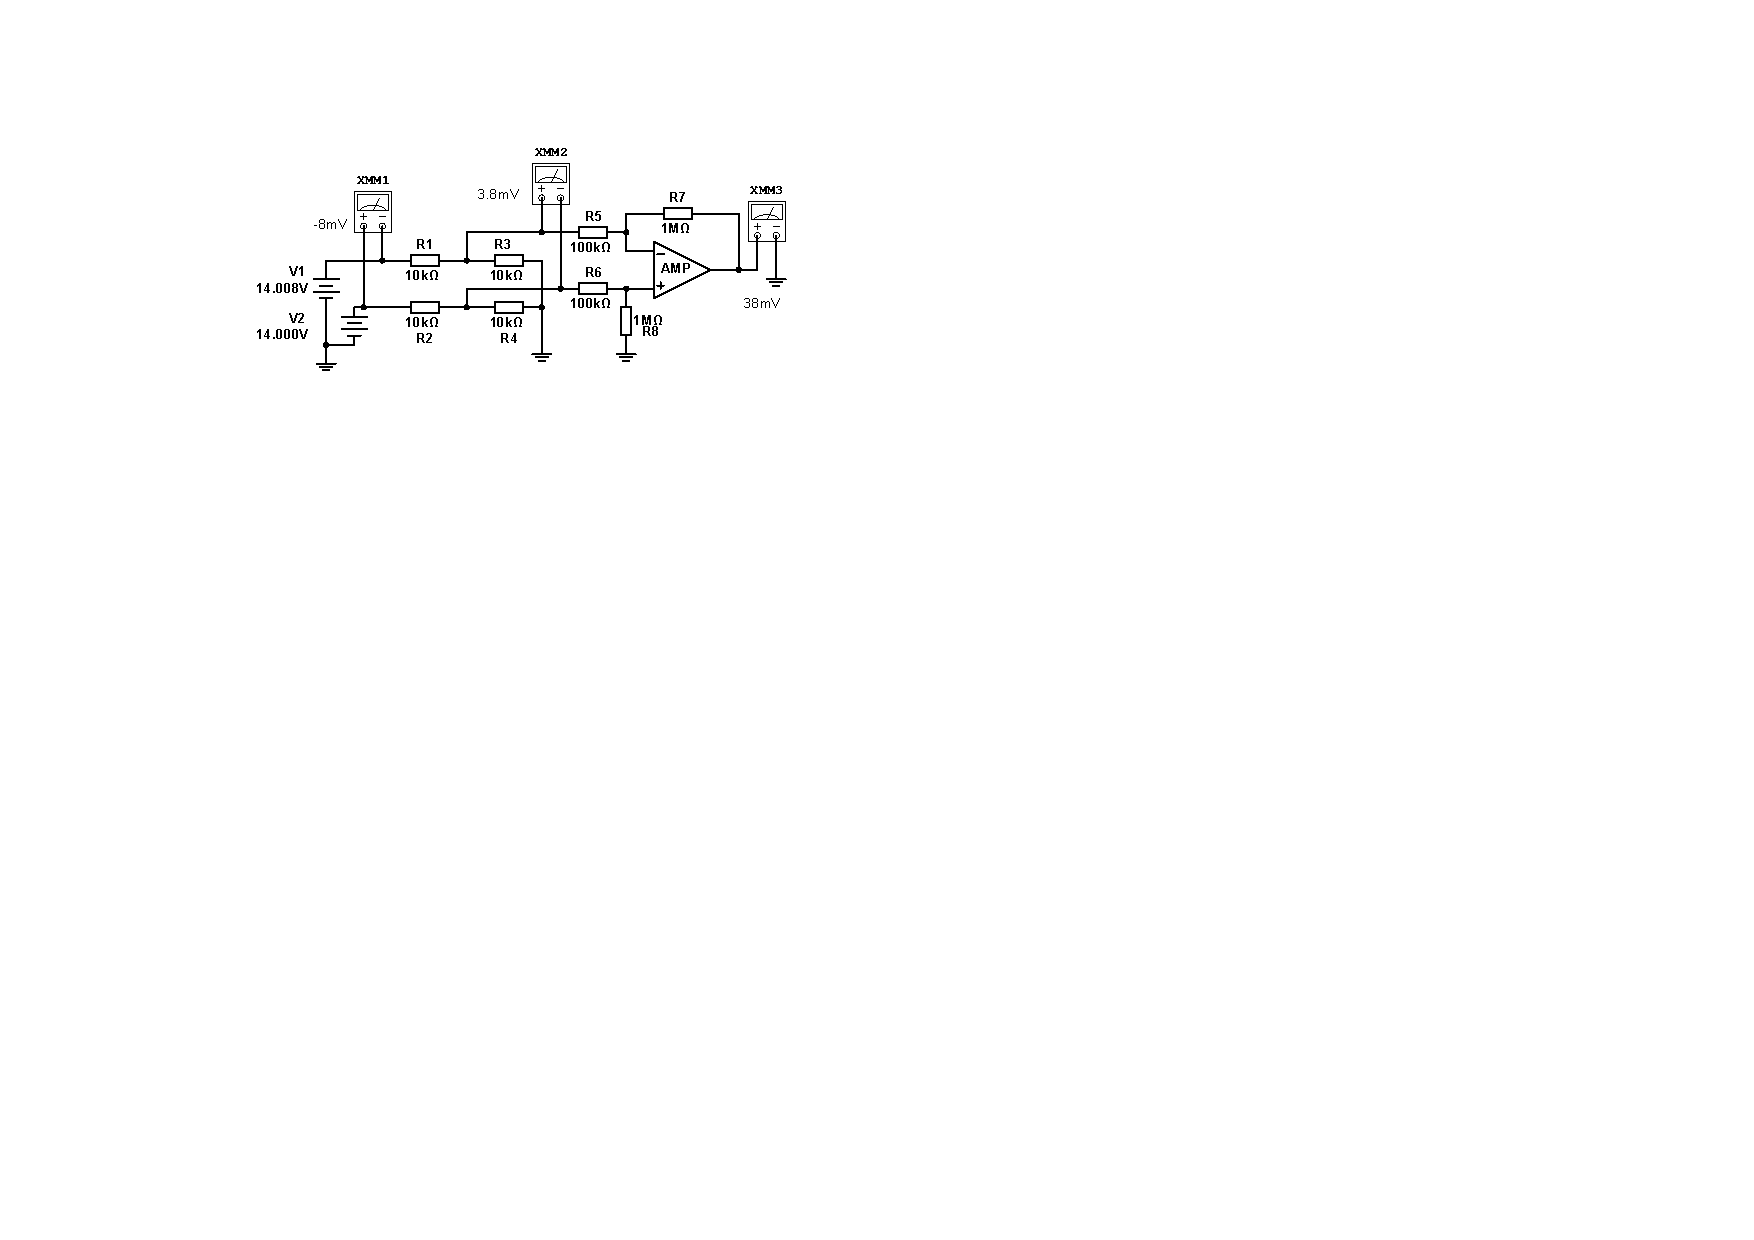
\includegraphics[scale=1.3]{Schaltung1.pdf}
	\caption{Schaltkonzept zur belastungsarmen Spannungsverstärkung der Hallspannung unter Berücksichtigung der oberen Spannungsgrenze der Ausgangsspannung des Operationsverstärkers. Für diese Widerstandswahl wird die Hallspannung $U_H=\SI{8}{\milli V}$ auf \SI{38}{mV} verstärkt.}
	\label{fig:schaltung}
\end{figure}
\noindent Mit dieser Schaltung ist es möglich, die Hallspannung mit einem Digitalmultimeter zu messen. Die Ausgangsspannung ist proportional zur Hallspannung, weshalb sie ebenfalls proportional zum Magnetfeld ist.\\

Für unsere Versuchsdurchführung steht das CASSY-Messgerät zur Verfügung, welches diesen Schritt vereinfacht, da es Spannungen in der gewünschten Auflösung direkt misst. Der Aufbau des obigen Schaltkonzepts ist in diesem Fall somit nicht nötig. Das CASSY Spannungsmessgerät misst mit einer Genauigkeit von \SI{0.01}{\milli V}.
\section{Durchführung und Auswertung}
\subsection{Versuchsdurchführung}
\label{sec:versuchsdurchfuhrung}
Bevor eine Messung gestartet werden kann, sind verschiedene Aspekte zu beachten. 
Die Offsets zwischen den Skalen der optischen Bänke zur Koordinatenunterlage wurden nach dem Aufbau des Versuches bestimmt, so dass bekannt ist, welche Einstellung des Lasers auf der Skala der optischen Bank welcher Position des Laserstrahls bezüglich der Skala Koordinatenunterlage entspricht (vgl. Abschnitt \ref{ch:abb}, Abb. \ref{fig:sk1}). Die Laser können dann mit einem Winkelmaß und einem Lineal, welches im rechten Winkel zur Tischebene aufgestellt wird, anhand der Skala der Koordinatenunterlage zueinander orthogonal und in gleicher Höhe parallel zur Tischebene ausgerichtet werden.\\

Diese Einstellungen sollten zwischen verschiedenen Messreihen überprüft werden, da es möglich ist, dass die Laser ihre Ausrichtung bei Stößen gegen den Aufbau ändern (Anforderung: Höhendifferenz in 1 Meter Abstand zum Laser: $\leq$ \SI{1}{\milli \meter}). Während der Messung werden die Laser auf den optischen Bänken parallel verschoben und mit maximal \SI{20}{\milli \ampere} versorgt, damit sie nicht überhitzen.\\

Zusätzlich muss bestimmt werden, auf welcher Position die Laser den Mittelpunkt der Spule markieren, um die absolute Position in der Spule im Raum zu erhalten. Dies kann bewerkstelligt werden, indem die (bereits orthogonal zueinander ausgerichteten) Laser auf der optischen Bank verschoben werden, bis sie gerade auf den Rand der Spule leuchten. Wird die Skalenposition des Lasers auf diese Weise auf den beiden Seiten des Spulenpaars bestimmt, kann durch Mittelwertbildung die Position bestimmt werden, die der Mitte der Spule in der jeweiligen Richtung entspricht. \\
\begin{figure}[H]
	\centering
	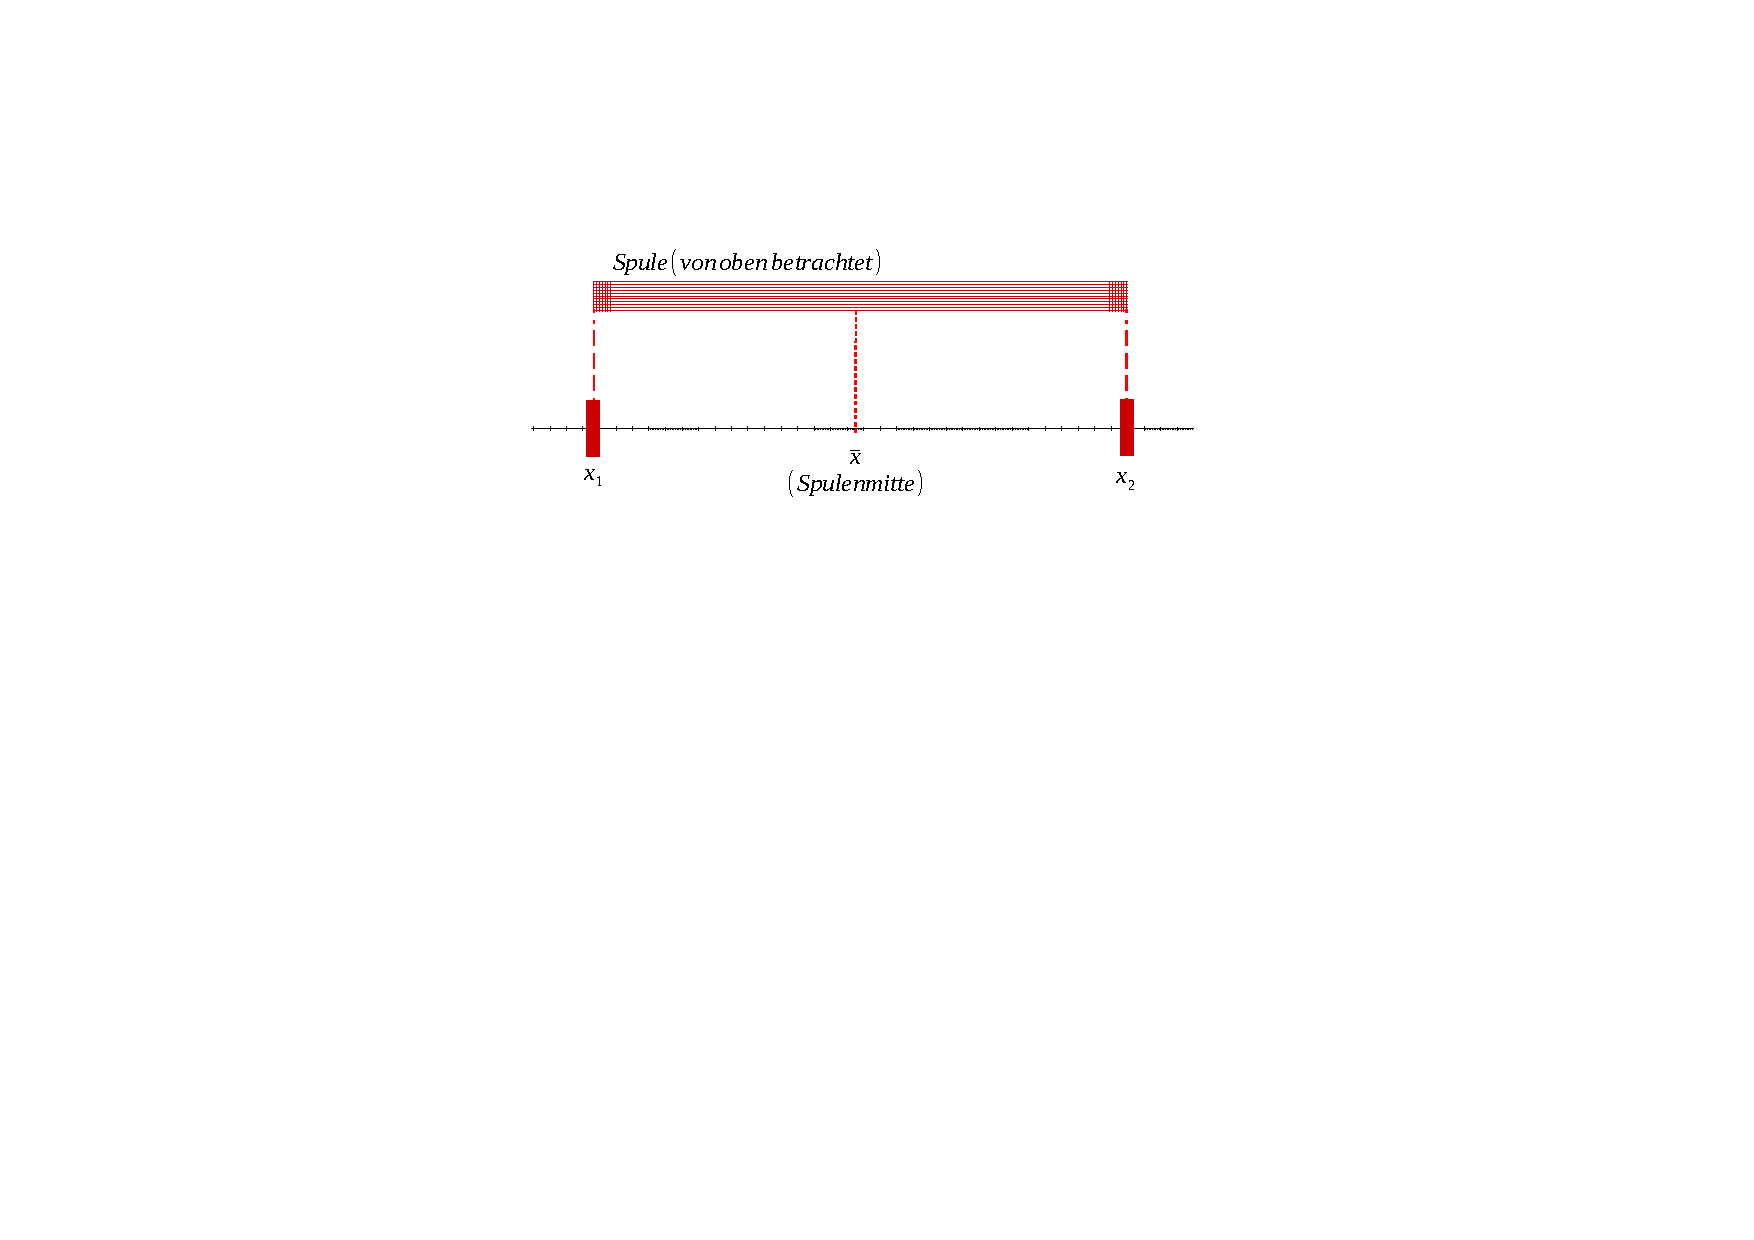
\includegraphics[scale=0.8]{pos1.pdf}
	\caption{Prinzipskizze zur Bestimmung der Position des Lasers auf der Skala der optischen Bank, die der Spulenmitte entspricht.}
	\label{fig:pos1}
\end{figure}

Die Spulen werden an die \SI{4.00(1)}{\ampere} und die Hallsonden an eine \SI{7.00(1)}{\milli \ampere} Konstantstromquelle angeschlossen. Zur Kontrolle der Ströme werden zusätzlich zwei Digitalmultimeter in Reihe geschaltet. Die Positionierung und Ausrichtung des Hallsensors erfolgt vor jedem Messwert mithilfe der bereits orthogonal zueinander ausgerichteten Laser. An der Halterung des Hallsensors wurde dafür ein Punkt markiert, welcher von einem Teil des Laserstrahls angeleuchtet werden muss, während der andere Teil die Sensorspitze erfasst. Dadurch wird gewährleistet, dass das Trägermaterial der Sonde parallel zum Laser (und somit auch zu den Spulen) verläuft. Die Messwerte werden dann nach einem vorgegebenen Raster nacheinander abgefahren, indem die Laser auf der optischen Bank verschoben und daraufhin der Sensor an die richtige Stelle gestellt wird. Dies ist in Abschnitt \ref{ch:abb} in Abbildung \ref{durchf3} zu sehen.\\

Ziel der Messungen ist es nun zunächst, den allgemeinen Feldverlauf des Spulenpaars zu bestimmen, und das Resultat mit dem Ergebnis der Simulation zu vergleichen. Spezieller soll erfasst werden, inwiefern das Feld im Inneren der Spulen homogen ist. Die Änderung der Homogenität bei verändertem Spulenabstand soll ebenfalls bestimmt werden.
\subsection{Resultate und Diskussion der Unsicherheiten}
Um Ergebnisse zu erhalten, die sich auswerten lassen, werden mit dem Sensor bestimmte Gebiete (Geraden, Ebenen) innerhalb und außerhalb der Spulen abgefahren. Zunächst wird dabei der Spulenabstand so gewählt, dass der Abstand $d$ zwischen den Spulen gleich ihrem mittleren Radius $\bar{r}=\SI{15.55(10)}{cm}$ ist. Anschließend wird der Abstand der Spulen verändert, um den Effekt auf das Magnetfeld betrachten zu können.
\subsubsection{Unsicherheit in der Positionsbestimmung}
Sowohl durch Ablesefehler als auch durch Aufbaufehler wird die Genauigkeit beeinflusst, mit der die Position des Sensors im Raum bestimmt werden kann. Im Folgenden soll deshalb die Unsicherheit in der Positionierung des Hallsensors abgeschätzt werden. Diese entsteht durch mehrere Einzelunsicherheiten:
\begin{itemize}
	\item Einfluss der Breite des Laserstrahls / Dimension der Sonden ($\sim\SI{1}{mm}$/ $\sim\SI{2}{mm}$, zusammen $\sim\SI{3}{mm}$)
	\item Ablesegenauigkeit auf der Skala der optischen Bank ($\sim\SI{0.5}{mm}$)
	\item Unsicherheit in der Differenz zwischen Position des Lasers und der gezeigten Position auf der Skala (der Laser ist durch seine Halterung um einige Millimeter nach rechts/links gegen die Skala verschoben) ($\sim\SI{0.5}{mm}$)
	\item Genauigkeit der horizontalen Position der Spule ($\sim\SI{1}{mm}$)
	\item Genauigkeit der z-Position (Höhe über der Tischplatte) der Spule ($\sim\SI{0.5}{mm}$) 
	\item Genauigkeit der Position der Laser in z-Richtung (zwischen $\SI{1}{mm}$ und $\SI{2}{mm}$)
	%\item Genauigkeit der Einstellbarkeit der Höhe des Lasers ($\sim\SI{2}{mm}$)
\end{itemize}
Insgesamt kann abgeschätzt werden, dass die bestimmte Position des Sensors im Raum relativ zur Spule in jeder Komponente um weniger als \SI{5}{mm} vom realen Wert abweicht ($\Delta x_i \simeq \SI{5}{mm}$).

\subsubsection{Qualitatives Ergebnis}
\label{qual}
Da zweidimensional (entlang einer Ebene) gemessene Datensätze zum einen eine hohe Zahl an Datenpunkten erfordern, und zum anderen schlecht grafisch auszuwerten sind, beschränken wir uns hierfür auf eine Messreihe in der x-y-Ebene durch den Koordinatenursprung (und somit auch durch den Schwerpunkt des Spulenpaars). Es wird ein Raster von diskreten Messpunkten innerhalb dieser Ebene mit dem Sensor abgefahren. Die Hallspannungen werden gemessen und das Magnetfeld mit Formel \ref{eq:B} bestimmt. Die Messpunkte werden zudem simuliert. Das Ergebnis ist in der folgenden Visualisierung als Vektorfeld zu sehen.
\begin{figure}[H]
	\centering
	\begin{subfigure}[c]{0.8\textwidth}
		\centering
		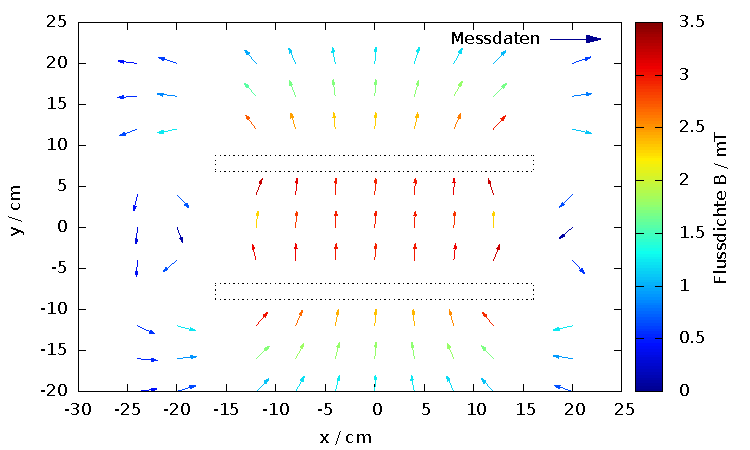
\includegraphics[scale=1.1]{exp_ebene.pdf}
		\caption{Experimentell bestimmtes Spulenmagnetfeld. Es ist eine leichte Neigung der Magnetfeldrichtung in positive x-Richtung zu erkennen (dazu später mehr). Der Feldverlauf und die Beträge des B-Feldes stimmen sehr gut mit den theoretischen Erwartungen überein.}
		\label{2da}
	\end{subfigure}
	\\
	\begin{subfigure}[c]{0.8\textwidth}
		\centering
		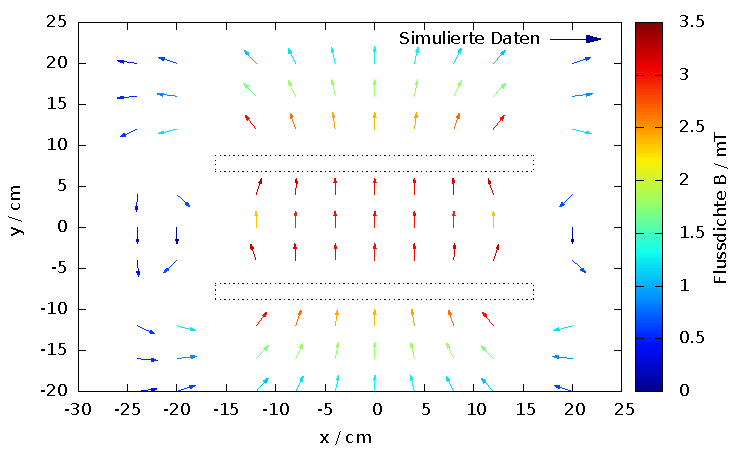
\includegraphics[scale=1.1]{sim_ebene.pdf}
		\caption{Theoretisch bestimmtes Spulenmagnetfeld. Die erwartete Homogenität des Feldes im Inneren ist gut zu erkennen.}
	\end{subfigure}
	\caption{Vergleich zwischen experimentellen und simulierten Daten. Der gestrichelte Umriss stellt die Position der Spulen dar.}
\end{figure}
Festzustellen ist, dass das Messresultat "`augenscheinlich"' gut mit der Simulation übereinstimmt. Dabei sind zwei Aspekte festzuhalten:
\begin{enumerate}
	\item Der Aufbau scheint nicht zu 100 \% gerade verschraubt worden zu sein, was die Neigung der Vektoren in x-Richtung erklärt. Hierauf wird in Abschnitt \ref{quant} genauer eingegangen.\footnote{Es wäre auch möglich, dass einer der Laser zur Positionierung durch einen Fehler leicht schief ausgerichtet wurde. Dies führt bezüglich der Relativposition zwischen Spule und Sensor auf das gleiche Ergebnis.}
	\item Größere Abweichungen sind vor allem an Stellen zu entdecken, an denen sich eine Komponente im Vorzeichen ändert, also der Vektor seine Richtung stark ändert, zum Beispiel bei (x, y)=($\SI{20}{cm}$, $\SI{0}{cm}$). Dies spielt eine Rolle in der Auswertung des Teils "`Parallele Richtung"' im nachfolgenden Abschnitt \ref{quant}.
\end{enumerate}
\subsubsection{Quantitatives Ergebnis}
\label{quant}
Um die Daten gut auswerten zu können, wird sich im Folgenden darauf beschränkt, eindimensionale Bereiche innerhalb der Spule zu untersuchen. Da das Verstellen der Laser zur Positionierung der Sonde nur in x- und y-Richtung schnell geht, beschränkt sich dies auf Geraden parallel zur xy-Ebene. Andere Geraden parallel zu einer Koordinatenachse verhalten sich aufgrund der Rotationssymmetrie des Systems äquivalent dazu.\\
\subsubsection*{Axiale Richtung (y)}
Die folgenden Abbildungen zeigen Messreihen für eindimensionale Datensätze entlang, bzw. parallel zur y-Achse. Man beachte die Änderung der Homogenität innerhalb der Spulen für veränderte z-Komponente.
\begin{figure}[H]
	
	\centering
	\begin{subfigure}[c]{0.8\textwidth}
	\centering
	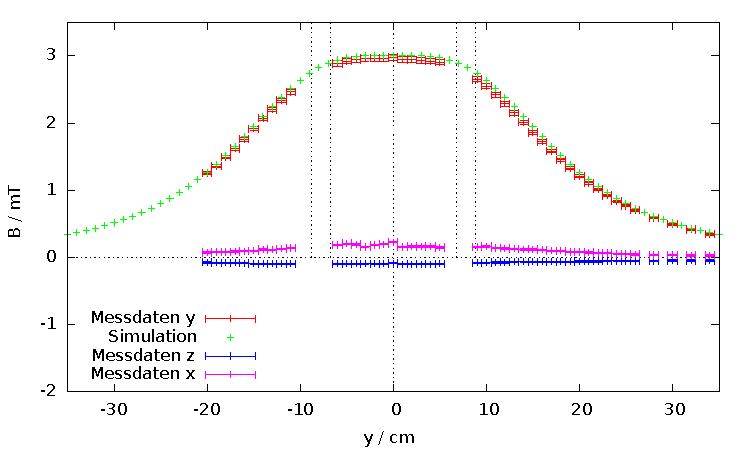
\includegraphics[scale=0.9]{abs1_Auswertung_Axial_1.pdf}
	\caption{$x=\SI{0}{cm}$, $z=\SI{0}{cm}$. Messwerte und simulierte Daten entlang der y-Achse. Die theoretischen Werte für die x- und z-Komponente des Magnetfeldes sind überall 0.}
	\end{subfigure}
	\\
	\begin{subfigure}[c]{0.8\textwidth}
		\centering
		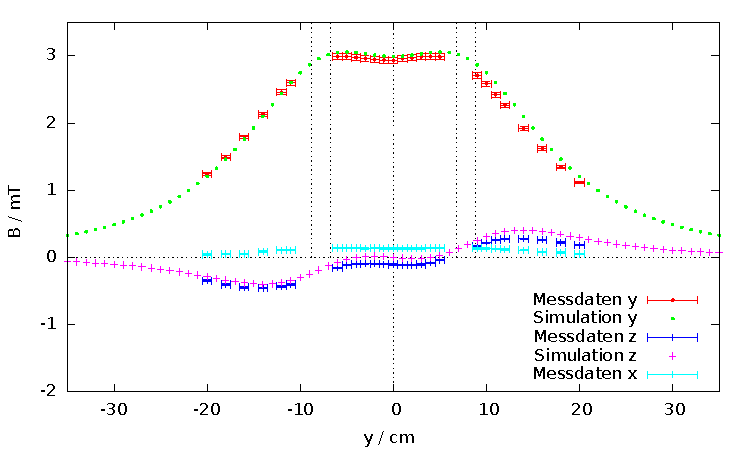
\includegraphics[scale=0.9]{abs1_Auswertung_Axial_2.pdf}
		\caption{$x=\SI{0}{cm}$, $z=\SI{5}{cm}$. Messwerte und simulierte Daten entlang einer Parallelen zur y-Achse. Die theoretische x-Komponente des Magnetfeldes ist überall 0. }
		\label{exp1a}
	\end{subfigure}
	\caption{Messergebnisse parallel zur y-Achse. Man erkennt die Homogenität innerhalb der Spulen, und den Abfall bei zunehmendem Radius. Es ist zu erkennen, dass das Feld in axialer Richtung homogen ist, und die Homogenität mit zunehmendem z abnimmt.}
	\label{fig:exp1}
\end{figure}
Die Messergebnisse bestätigen die Theorie innerhalb der statistischen Unsicherheiten weitestgehend. Leichte Abweichungen zwischen Theorie und Messung zeigen sich in Abb. \ref{exp1a} in der x-Komponente des Magnetfeldes. Hier liegt offenbar ein systematischer Messfehler zugrunde. (xXxXxErklärung?xXxXx)
\subsubsection*{Parallele Richtung}
Eine analoge Messung des Magnetfeldes wurde entlang und parallel zu der x-Achse parallel zu den Spulen durchgeführt. Da diese Ebene die entscheidende für z.B. den Versuch des "`Fadenstrahlrohrs\footnote{z.B. beim Anfängerpraktikum Physik, BUW}"' darstellt, wurden hierzu mehrere Messungen für verschiedene Höhen z der Messung durchgeführt. Die Ergebnisse hierzu werden im Folgenden grafisch dargestellt.
\begin{figure}[H]
	\centering
	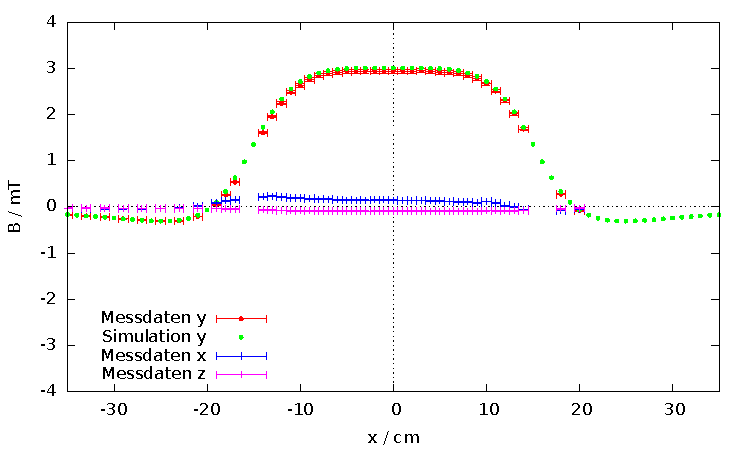
\includegraphics[scale=1.1]{abs1_Auswertung_parallel_1.pdf}
	\caption{Verlauf des Magnetfeldes entlang der x-Achse mit z=x=0. Die theoretische x- und z-Komponente des B-Feldes ist konstant 0.}
	\label{fit:par1}
\end{figure}
Die Messwerte stimmen innerhalb der statistischen Unsicherheiten mit den theoretischen Erwartungen überein. Man kann erkennen, dass das Feld in y-Richtung ca. $\pm \SI{5}{cm}$ um den Ursprung der Spule herum sehr homogen ist. Das Fadenstrahlrohr zu diesen Spulen erlaubt maximal einen Radius des Fadenstrahls von ca. \SI{5}{cm}. Mit diesen Messdaten ist es möglich zu sagen, dass das Magnetfeld in diesem Bereich sehr homogen ist, und die im Praktikum getätigten Annahmen somit gültig sind. Auch bei dieser Messung ist zu bemerken, dass die x-Komponente des Magnetfeldes mehr abweicht als um die statistische Unsicherheit.\\

In den Abbildungen \ref{fig:p2} bis \ref{fig:p5} in Abschnitt \ref{ch:abb} ist die Messreihe für verschiedene Geraden parallel zur x-Achse abgebildet. Dort ist zu erkennen, wie die horizontale Homogenität des Feldes mit zunehmender z-Komponente abnimmt. Auch in diesen Messungen verhält sich die x-Komponente, und mit zunehmendem z auch die z-Komponente des Magnetfeldes anders als die Simulation es vorhersagt.\\

\noindent \textbf{Systematische Fehler}\\
Alle Messungen in diesem Abschnitt haben eine gemeinsame systematische Unsicherheit: Ihre x-Komponente des Magnetfeldes verhält sich der Form nach punktsymmetrisch um den Ursprung mit einer zusätzlichen Verschiebung nach oben. Eine solche x-Koordinate ist zu erwarten, wenn man eine kleine Verschiebung in der y-Position des Sensors annimmt. Dies ist in Abbildung \ref{plot0} zu sehen.
\begin{figure}[H]
	\centering
	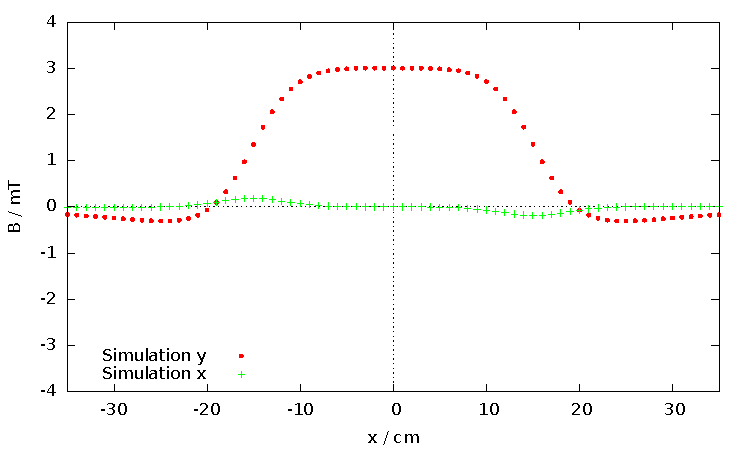
\includegraphics[scale=0.9]{plot0.pdf}
	\caption{Theoretischer Feldverlauf entlang der x-Achse, wenn mit $y=\SI{5}{mm}$ eine Abweichung innerhalb der Fehler in der y-Position angenommen wird.}
	\label{plot0}
\end{figure}
Es ist somit möglich, dass der Verlauf des Feldes in x-Richtung durch eine solche Positionsunsicherheit zustande kommt. Die Verschiebung nach oben kann zum Teil durch eine Versetzung der Spulen gegeneinander erklärt werden. Der Spulenaufbau wurde bislang als ideal betrachtet. Verschiebt man in der Simulation jedoch die Spulen gegeneinander in x-Richtung, ergibt sich eine Verschiebung nach oben bzw. unten. Dieser Ansatz kann diese Abweichung aber nur teilweise erklären, da die nötige Verschiebung für die gemessene Abweichung über $\SI{1}{cm}$ betragen würde. Eine so große Abweichung der Spulen gegeneinander kann allerdings ausgeschlossen werden. Die Ursache dieses systematischen Fehlers kann von uns an dieser Stelle nicht genauer eingegrenzt werden.\\

Die systematische Abweichung in der x-Komponente wird größer, je weiter die Messung von der x-Achse entfernt gewesen ist. Dies hängt mit dem zweiten systematischen Fehler zusammen: Dem Verhalten der z-Komponente für "`große"' z. Wie in Abbildung \ref{fig:p5} zu sehen ist, sind y- und z-Komponente an einigen Stellen betragsmäßig fast gleich groß, obwohl theoretisch zu erwarten ist, dass die z-Komponente konstant Null ergibt. Dies lässt sich mit dem in Abschnitt  \ref{qual} unter Punkt 2 genannten Aspekt erklären. Erhöht man die z-Koordinate, gelangt die Messung in Bereiche des Magnetfeldes, die sich stark in ihrer Richtung ändern. So kann eine sehr kleine Unsicherheit in der Position eine starke Abweichung einer oder mehrerer Komponenten des Magnetfeldes von der Theorie bedeuten (vgl. Abb. \ref{2da} bei (x, y)=($\SI{20}{cm}$). Es ist also schwer möglich, diese Art von systematischen Fehlern zu verhindern, wenn die Position des Hallsensors im Raum relativ zu den Spulen nicht genauer bekannt ist.
\subsubsection*{Temperaturabhängigkeit der Hallspannung}
Die verwendeten Hallsensoren vom Typ KSY 44 besitzen einen Temperaturkoeffizienten, der bestimmt, wie sich die Hallspannung in Abhängigkeit der Temperatur ändert. Dieser beträgt $\Delta U_T \simeq -0.03\ \% / \text{K}$. Es kann somit festgehalten werden, dass dieses Verhalten der Sonden keinen Einfluss auf die Messungen haben kann, da die Temperatur während des Versuches überwacht wurde und sich nicht um mehr als \SI{2}{\kelvin} geändert hat.
\subsubsection{Änderung des Spulenabstands}
Es konnte zuvor gezeigt werden, dass das Magnetfeld eines Helmholtzspulenpaars im Inneren der Spulen sehr homogen verläuft. Nun soll untersucht werden, ob und wie diese Eigenschaft vom Abstand zwischen den Spulen abhängt. Dazu werden analoge Messreihen zu den vorherigen mit verdoppeltem Spulenabstand d=\SI{31.1(2)}{cm} durchgeführt.
\begin{figure}[H]
	\centering
	\begin{subfigure}[c]{0.46\textwidth}
		\centering
		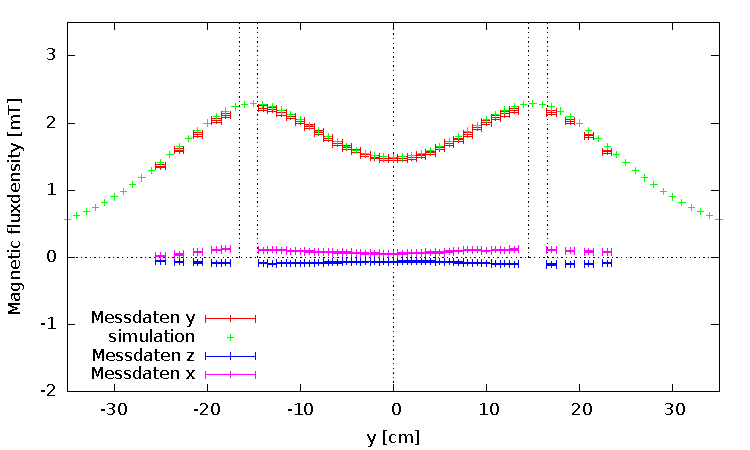
\includegraphics[scale=0.6]{plot_neuer_abstand_1.pdf}
		\caption{Magnetfeld entlang der y-Achse.}
	\end{subfigure}
\hspace{0.04\textwidth}
	\begin{subfigure}[c]{0.46\textwidth}
		\centering
		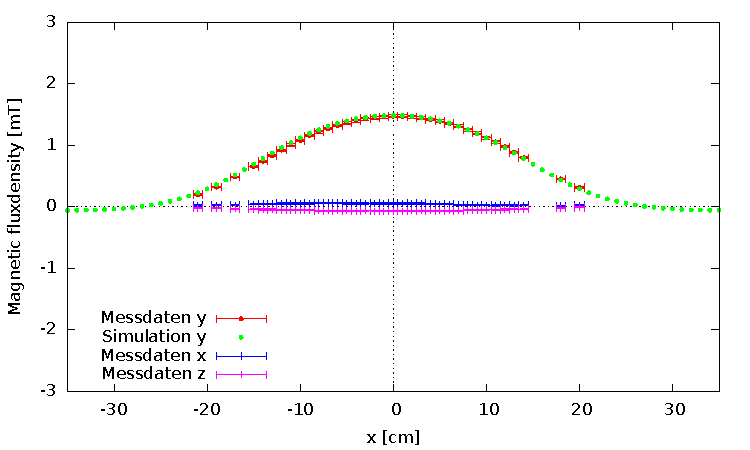
\includegraphics[scale=0.6]{plot_neuer_abstand_2.pdf}
		\caption{Magnetfeld entlang der x-Achse.}
	\end{subfigure}
	\caption{Magnetfeldverlauf entlang der x- und y-Achse nach Verdopplung des Spulenabstandes. Im Inneren der Spulen ist das Feld nicht mehr homogen. Die theoretischen x- und z-Komponenten des Magnetfeldes sind konstant Null.}
\end{figure}
Man erkennt also, dass die Bedingung, dass der Abstand der Spulen zueinander ihrem Radius entspricht, wesentlich ist für die Homogenität im Inneren der Spulen. In den Abbildungen \ref{fig:p6} bis \ref{fig:p8} sind weitere Messdaten für $z> 0$ zu sehen. Auch dort ist beobachtbar, dass die systematische Abweichung für größeres z ansteigt. Dies wurde bereits im vorherigen Abschnitt diskutiert.
\subsubsection*{Simulation eines kleineren Abstandes}
Schlussendlich soll mit der nun experimentell bestätigten Theorie ein geringerer Spulenabstand simuliert werden, um zu überprüfen, wie sich dies auf die Homogenität auswirkt. Im Folgenden ist das Simulationsergebnis für den Feldverlauf entlang der x- und y-Achse zu sehen, bei einem Abstand vom halben mittleren Spulenradius $\frac{\bar{r}}{2}=\SI{7.78(5)}{cm}$.
\begin{figure}[H]
	\centering
	\begin{subfigure}[c]{0.46\textwidth}
		\centering
		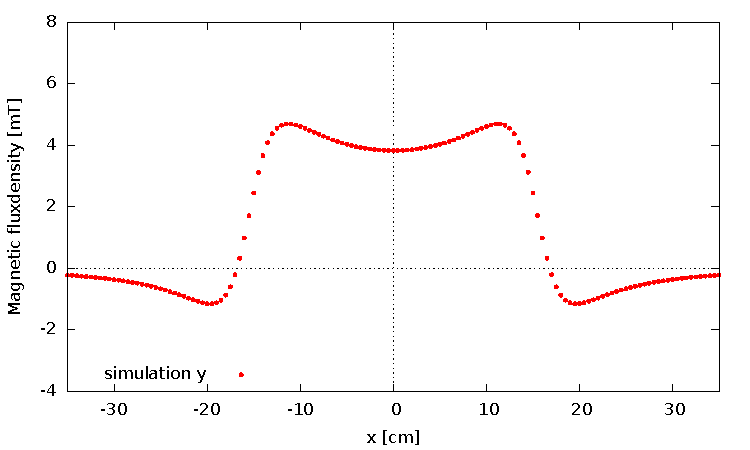
\includegraphics[scale=0.6]{plot00.pdf}
		\caption{Entlang der x-Achse.}
	\end{subfigure}
	\hspace{0.04\textwidth}
	\begin{subfigure}[c]{0.46\textwidth}
		\centering
		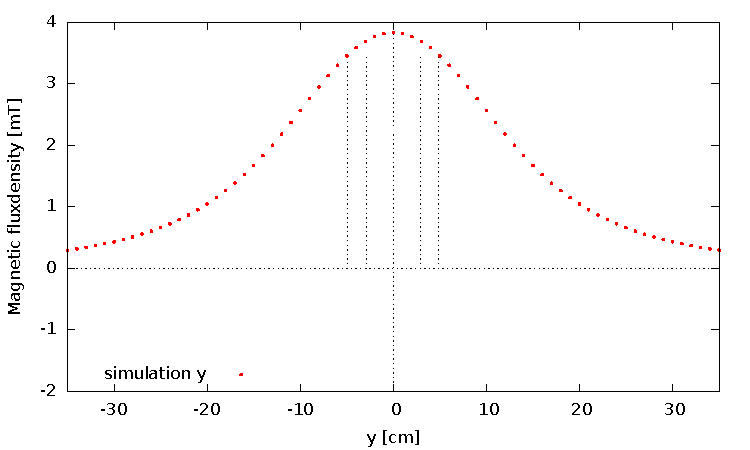
\includegraphics[scale=0.6]{plot01.pdf}
		\caption{Entlang der y-Achse.}
	\end{subfigure}
\caption{Simulierter Verlauf des Magnetfeldes für halben Spulenabstand im vergleich zur Helmholtzkonfiguration. Jeweils gezeichnet ist nur die y-Komponente. Die $B_x$ und $B_y$ sind identisch 0.}
\end{figure}
Wie man sieht, ist das Magnetfeld für den geringeren Spulenabstand ebenfalls nicht mehr homogen. Es kann also bestätigt werden, dass die Gleichheit von Abstand und Radius der Spulen notwendig ist für die Homogenität im Inneren des Spulenpaars.
\section{Fazit und Evaluation}
\subsection{Zusammenfassung der Ergebnisse}
Im Folgenden werden die wichtigsten Ergebnisse der Versuchsreihe zusammengefasst.
\begin{itemize}
	\item Es ist möglich, durch drei orthogonal zueinander positionierte Hallsonden einen Hallsensor zu bauen, der das Magnetfeld vektoriell misst. Beim Aufkleben der Sonden ist es wichtig, keine Inklination zwischen den Sonden zu produzieren.
	\item Das Magnetfeld eines Spulenpaars in Helmholtzkonfiguration ist im Spuleninneren nahezu homogen. In paralleler Richtung durch das Spulenzentrum ergibt sich bei einem Spulenradius von \SI{15.55}{cm} ein homogener Bereich mit einem Radius von ca. \SI{5}{cm}.
	\item Zum Ausmessen eines Feldes mit dem Hallsensor ist es essentiell, die Position des Sensors relativ zur Spule zu kennen. Bereits kleine Abweichungen führen dazu, dass einzelne Komponenten des Magnetfeldes starke systematische Unsicherheiten erhalten, wenn in einem Feldbereich mit hohem Gradienten gemessen wird.
	\item Statische Magnetfelder lassen sich theoretisch sehr gut vorhersagen und berechnen.
\end{itemize}
\subsection{Bewertung: Haben wir unser Ziel erreicht?}
\newpage
\section{Anhang}
\begin{singlespace}
\subsection{Python-Programm zur numerischen Berechnung des Spulenmagnetfeldes}
\label{ch:code}
Im Folgenden ist der Sourcecode (Python Ver. 3) zur numerischen Integration von Formel \ref{eq:Btheo} beispielhaft für eine Iteration über die x-y-Ebene gezeigt.
\begin{center}
	\textbf{Code 1:} Biot\_Savart\_reale\_Spule.py
\end{center}
\begin{lstlisting}
from scipy.integrate import tplquad # Lib fuer numerische Integration
import numpy as np
import math
import multiprocessing as mp

# Definition der Integrale in Komponenten (vgl. )
def fnx(r,p,w,x,y,z,j,m):
   return ((j*m*r / (4*math.pi)) * (np.cos(p)*(y-w)) \
   / ( ( ((x)-r * np.cos(p))**2 +((-z)-r*np.sin(p))**2 \
   + (y-w)**2 )**(1.5) ))

def fnz(r,p,w,x,y,z,j,m):
   return ((j*m*r / (4*math.pi)) *(-1) * (np.sin(p)*(y-w)) \
   / ( ( ((x)-r * np.cos(p))**2 +((-z)-r*np.sin(p))**2 \ 
   + (y-w)**2 )**(1.5) ))

def fny(r,p,w,x,y,z,j,m):
   return ((j*m*r/(4*math.pi))*(r-(((-z)*np.sin(p))+((x)*np.cos(p)))) \ 
   / ( ( ((x)-r * np.cos(p))**2 +((-z)-r*np.sin(p))**2 \
   + (y-w)**2 )**(1.5) ))

# Definition der noetigen Parameter und Variablen
x=y=z=0.0
Q=0.155/2     # Halber Spulenabstand/2
ri=0.150      # Innenradius
dr=0.011      # Radiale Dicke bis zum Aussenradius
ra=ri+dr      # Aussenradius
d=0.02        # Breite
i=4.00        # Strom
n=130         # Windungszahl
j=i*n/(d*dr)  # Stromdichte ueber Spulenquerschnitt
# Konstanten 
m = 1.256637061e-6  # Feldkonstante
length = 1          # Vektor-Einheitslaenge

# Integrationsgrenzen fuer Volumenintegral
aw=-d/2 
bw= d/2
ap=0.0
bp=2*math.pi 
ar=ri
br=ra
# Trivialfunktionen fuer Multiprocessing
# (Ersatz fuer Lambda-Funktion, die zusammen mit Multiprocessing
# Probleme beim internen pickling verursacht)
def f1(abc):
   return ap

def f2(abc):
   return bp

def f3(abc, cde):
   return ar

def f4(abc, cde):
   return br

for s in range(-7, 8):    # Iteration ueber die Spulen in x-Richtung
   x=s/35
   print("----------- S = ", s)
   for t in range(-7, 8): # Iteration in y Richtung
      y1=(t/35)-Q
      y2=(t/35)+Q
      y=t/35
      print("- T = ", t)
      pool=mp.Pool(6)
      
      results1=pool.starmap(tplquad, [\   # Numerische Integration
      (fnx, aw, bw, f1, f2, f3, f4,\      # fuer 1. Spule
      (x, y1, z, j, m), 4.49e-06, 1.49e-04), \
      (fny, aw, bw, f1, f2, f3, f4, \
      (x, y1, z, j, m), 4.49e-06, 1.49e-04), \
      (fnz, aw, bw, f1, f2, f3, f4, \
      (x, y1, z, j, m), 4.49e-06, 1.49e-04)])
      
      results2=pool.starmap(tplquad, [\   # Numerische Integration 
      (fnx, aw, bw, f1, f2, f3, f4, \     # fuer 2. Spule
      (x, y2, z, j, m), 4.49e-06, 1.49e-04), \
      (fny, aw, bw, f1, f2, f3, f4, \
      (x, y2, z, j, m), 4.49e-06, 1.49e-04), \
      (fnz, aw, bw, f1, f2, f3, f4, \
      (x, y2, z, j, m), 4.49e-06, 1.49e-04)])
      
      pool.close()
      pool.join() # Auf Ergebnisse der einzelnen Prozesse Warten
      Ix=results1[0][0] + results2[0][0]  # Superposition der Felder 
      Iy=results1[1][0] + results2[1][0]  # (Ergebnis)
      Iz=results1[2][0] + results2[2][0] 
      # Speichern des Datenpunkts
      tf = open( 'datafile2.txt', 'a')
      tf.write(repr(x)+" " +repr(y) +" "+repr(z) + " "+ \
      repr(Ix*length/abs) + " " + repr(Iy*length/abs) + " " + \
      repr(Iz*length/abs)+ " " + repr(abs) +'\n') 
      tf.close() 
\end{lstlisting}
\end{singlespace}
\newpage
\subsection{Abbildungen}
\label{ch:abb}
\begin{figure}[H]
\centering
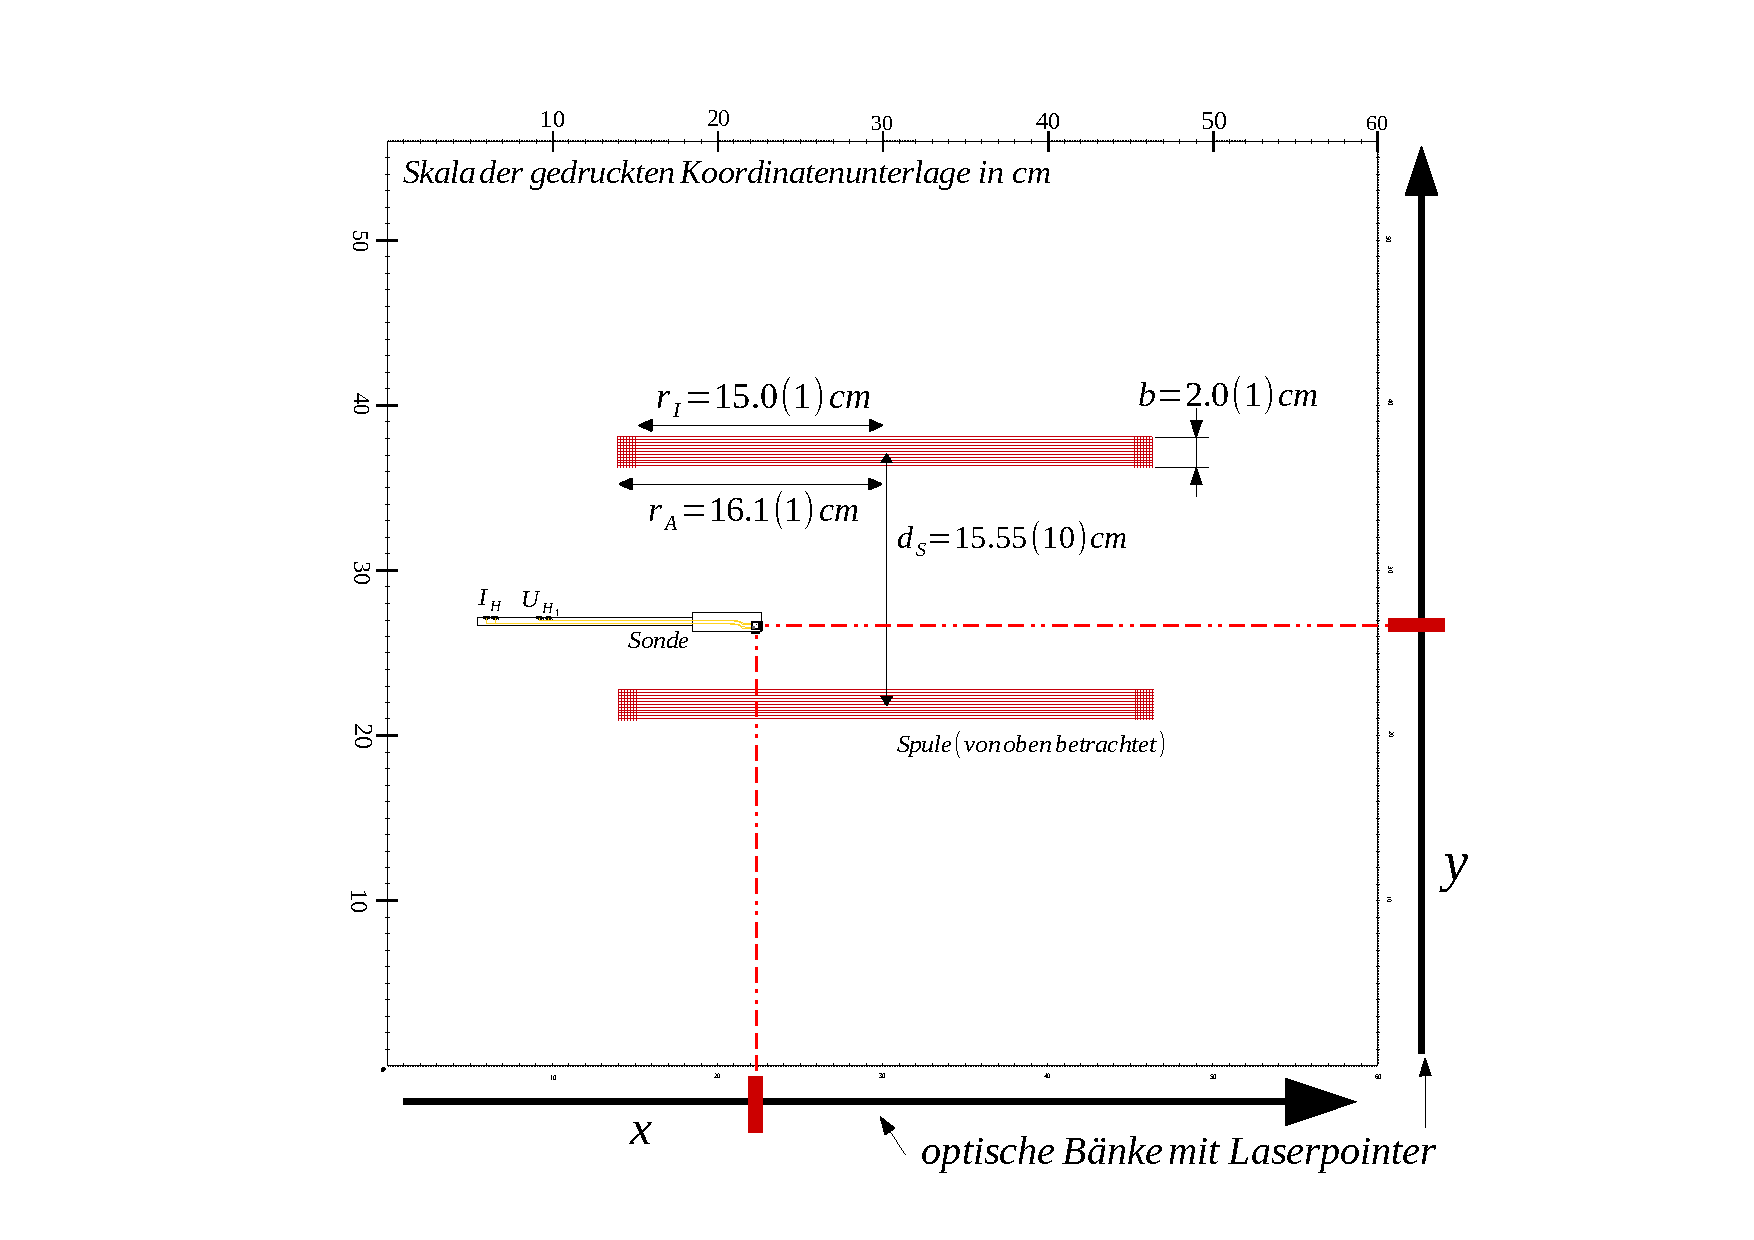
\includegraphics[scale=0.85]{Aufbauskizze1.pdf}
\caption{Prinzipskizze des Messaufbaus. Die Ansicht ist von oben. Das Spulenpaar (rot) wird von einer Skala und zwei optischen Bänken umschlossen. Die Optischen Bänke tragen Laserdioden, die zur Anpeilung der Sonde dienen. Vor der Messung muss die innere Skala mit der Skala der optischen Bank angeglichen werden, sowie die Laser mithilfe dieser Skalen senkrecht zueinander und parallel bzw. senkrecht zu den Spulen ausgerichtet werden.}
\label{fig:sk1}
\end{figure}
\newpage
\begin{figure}
	\centering
	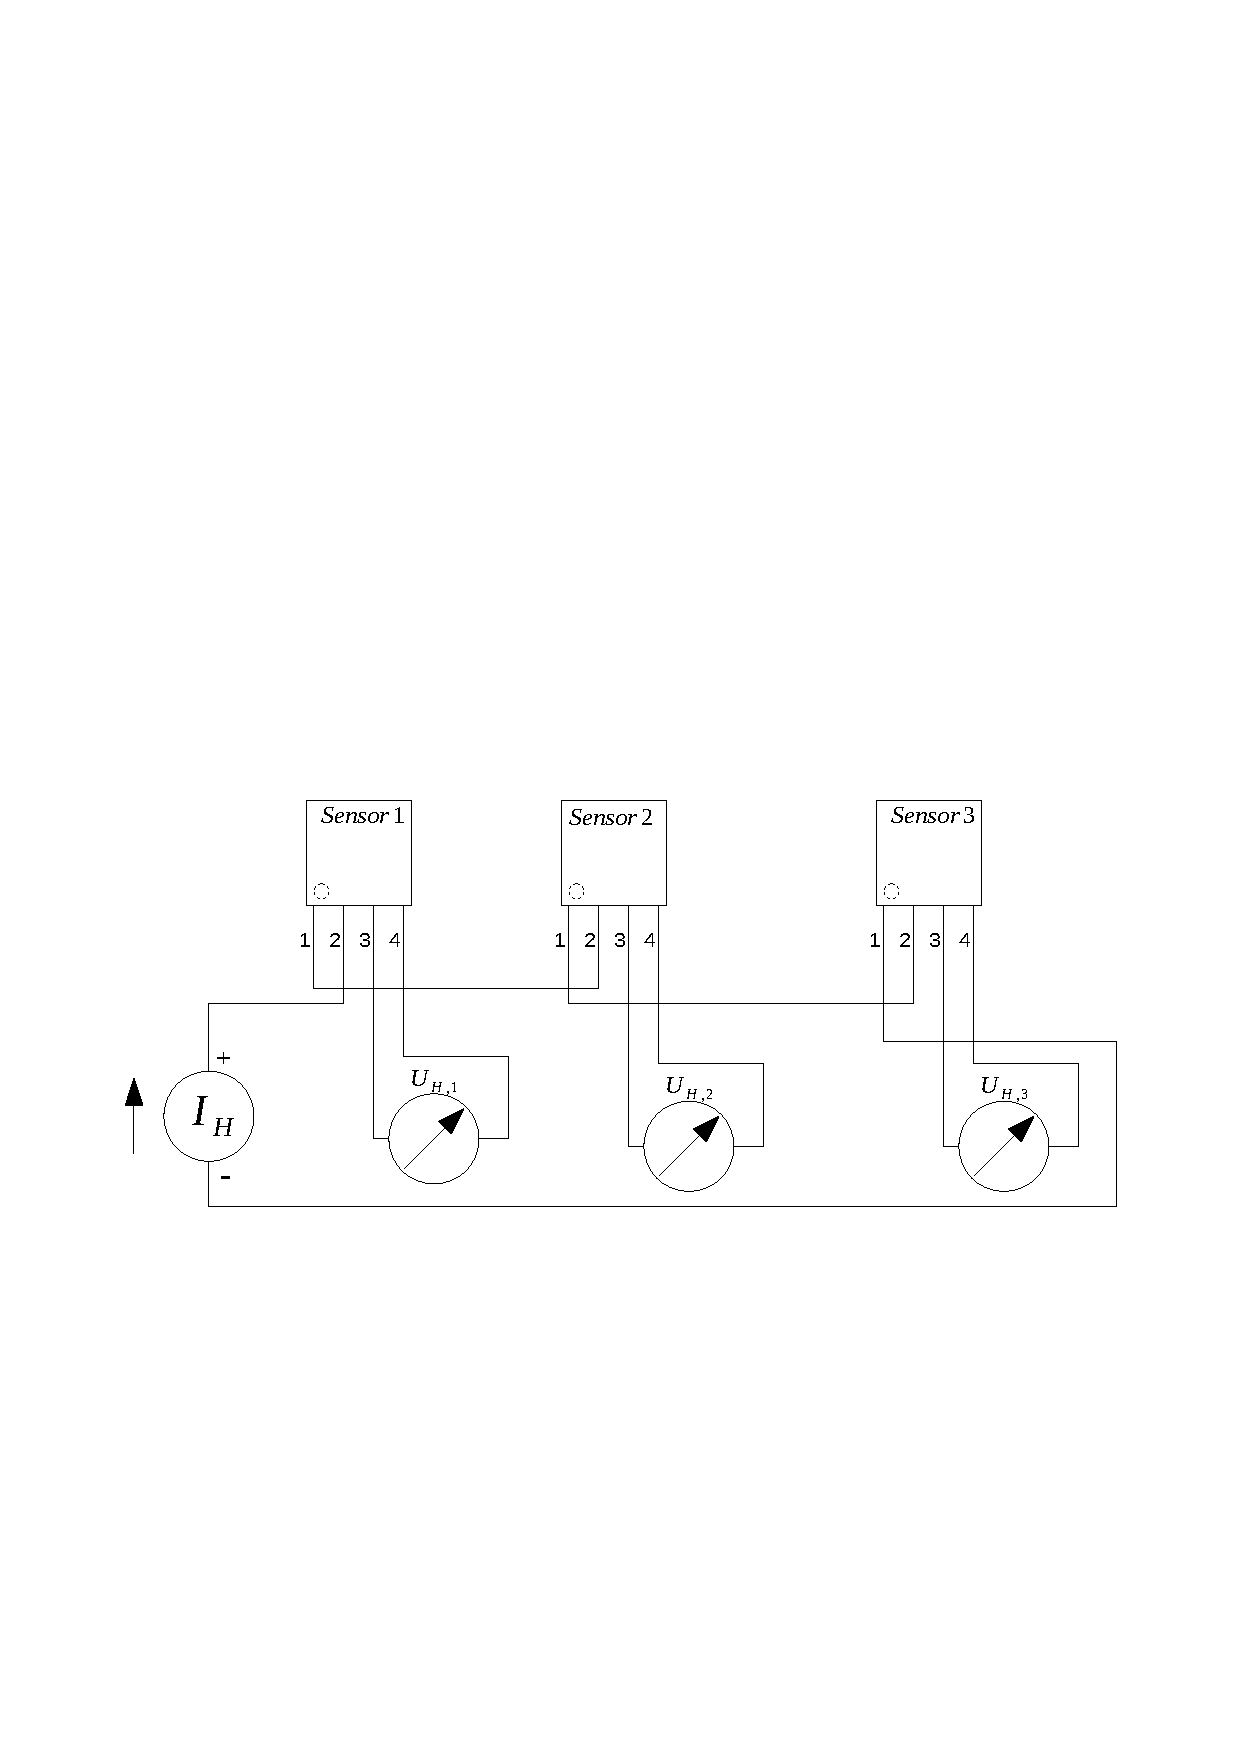
\includegraphics[scale=0.8]{Hall-Sensoren-Schaltung.pdf}
	\caption{Schaltplan der Hallsonden. Der Versorgungsstrom wird in Reihe geschaltet, weshalb die Ausgänge der hallspannungen auf einem Potential zwischen 0 und 20 V liegen.}
	\label{sch-sond}
\end{figure}
\begin{figure}
	\centering
	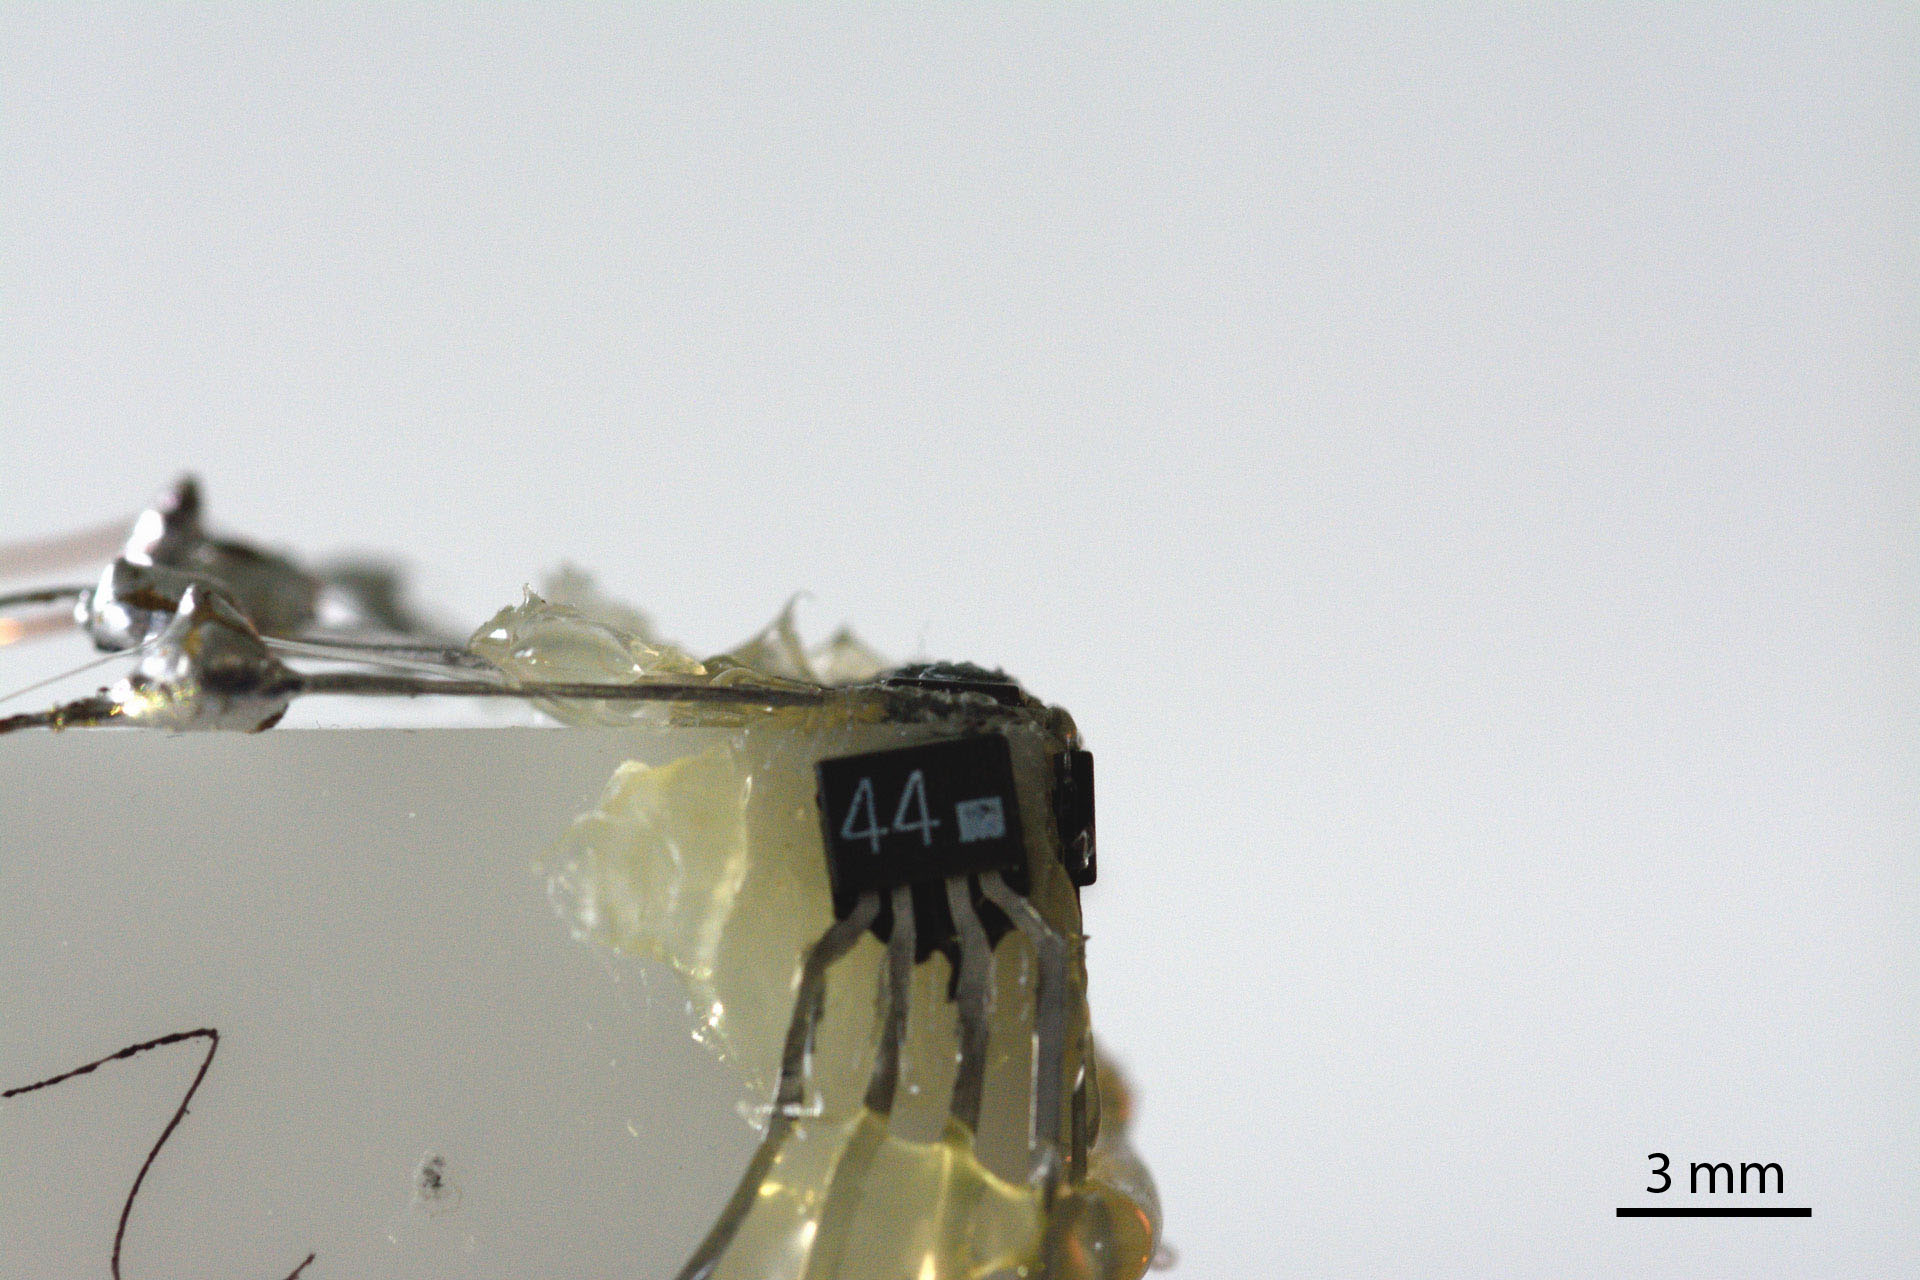
\includegraphics[scale=0.2]{sensor.jpg}
	\caption{Makroaufnahme der angeklebten und gelöteten Hallsonden auf das Trägermaterial. Bei genauem hinsehen erkennt man die leichte (in der Auswertung vernachlässigte) Inklination der Hallsonden oben und rechts.}
	\label{sond-foto}
\end{figure}
\begin{figure}[H]
	\centering
	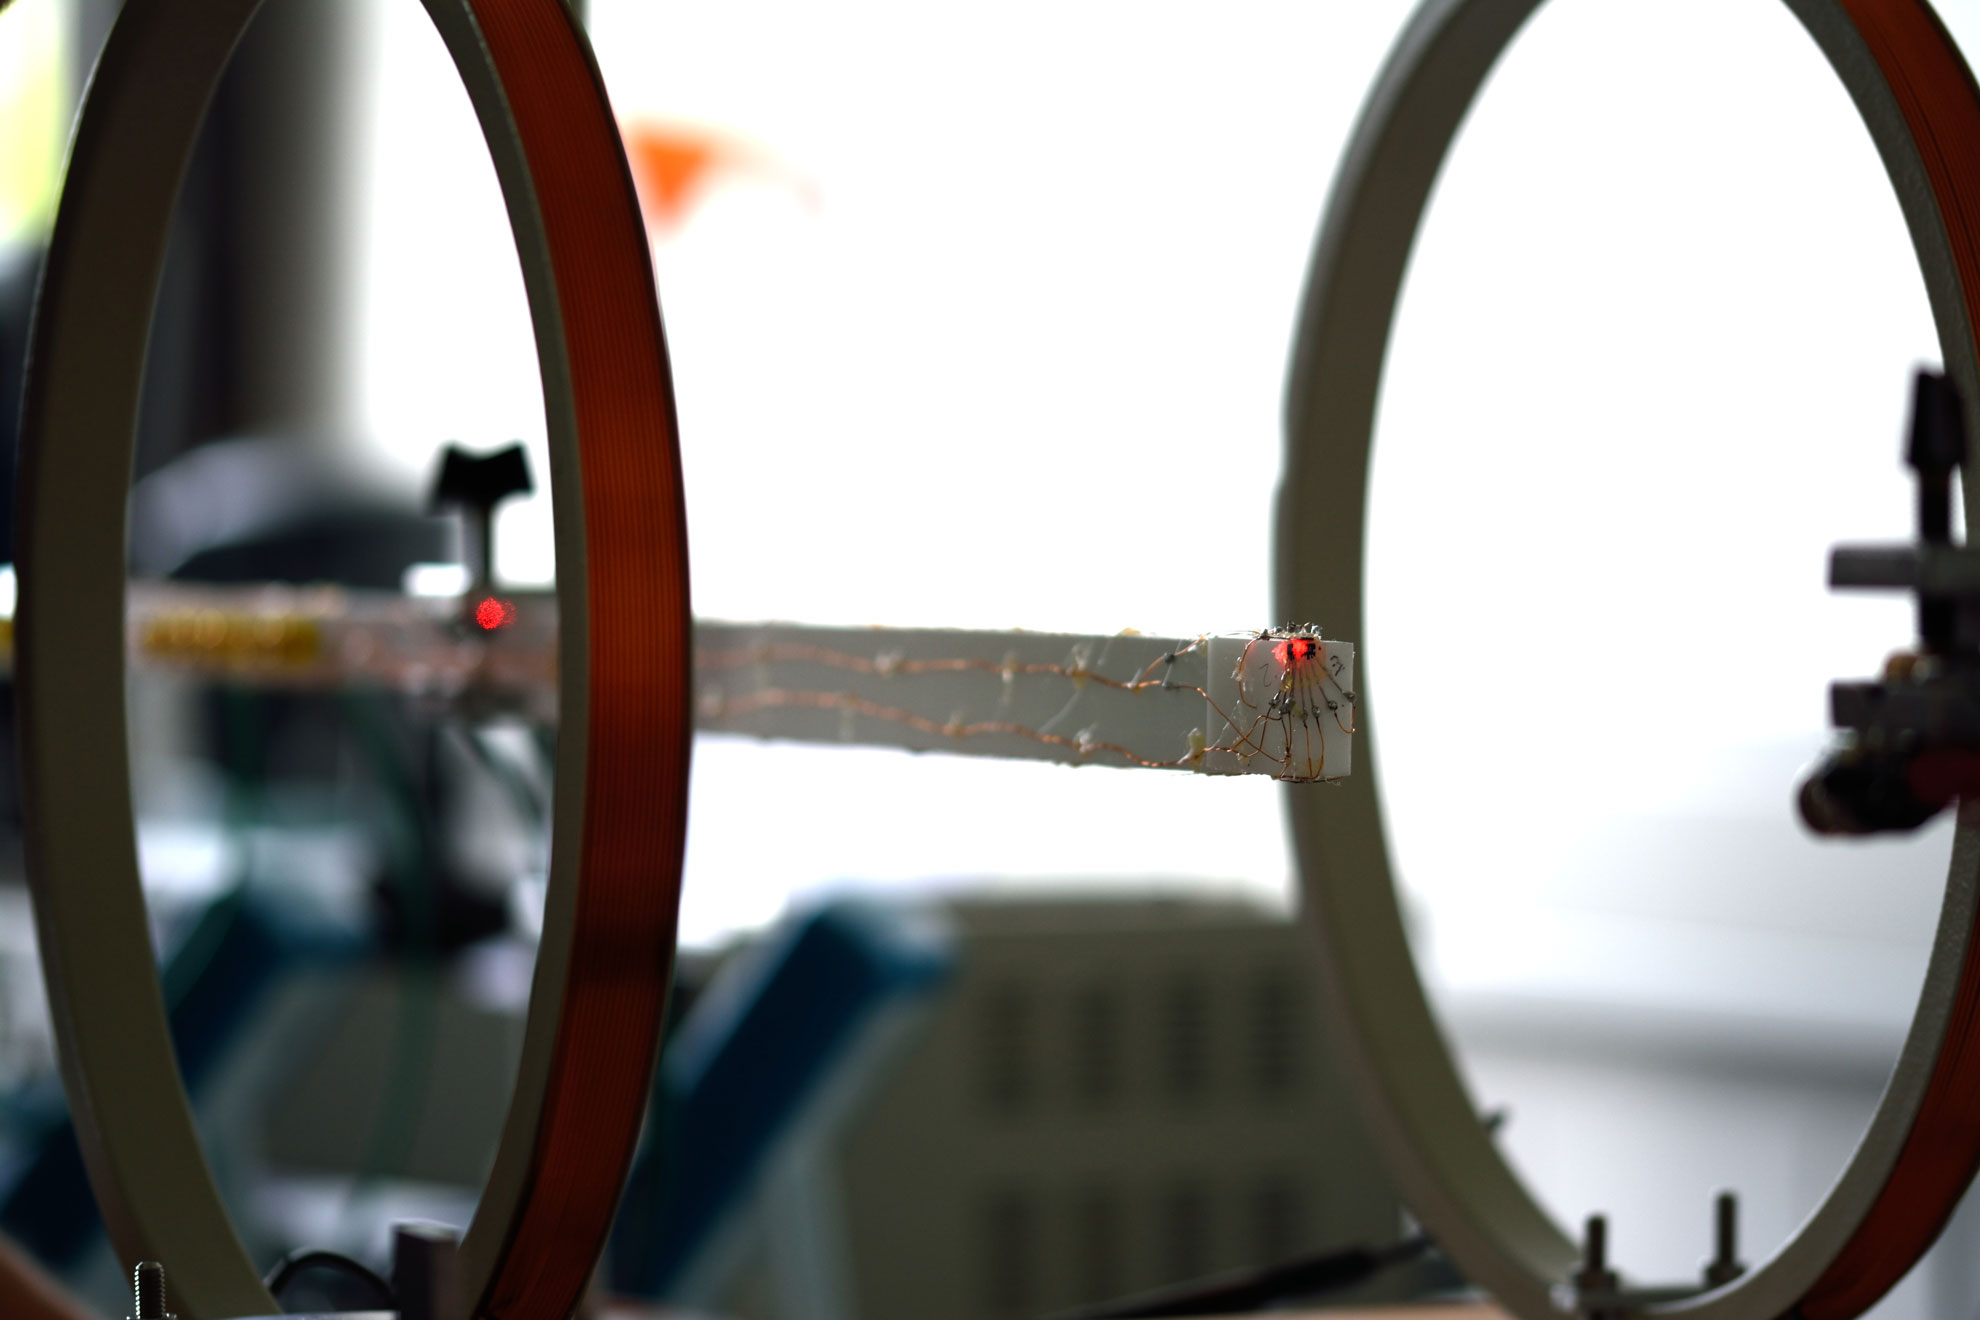
\includegraphics[scale=0.19]{durchfuehrung2.jpg}
	\caption{Versuchsaufbau während einer Messung. Es lassen sich die zwei Stellen erkennen, wo Laserlicht reflektiert wird. Auf diese Weise wird gewährleistet dass die Sonde parallel zum Laser / zu den Spulen gehalten wird.}
	\label{ph:1}
\end{figure}
\begin{figure}[H]
	\centering
	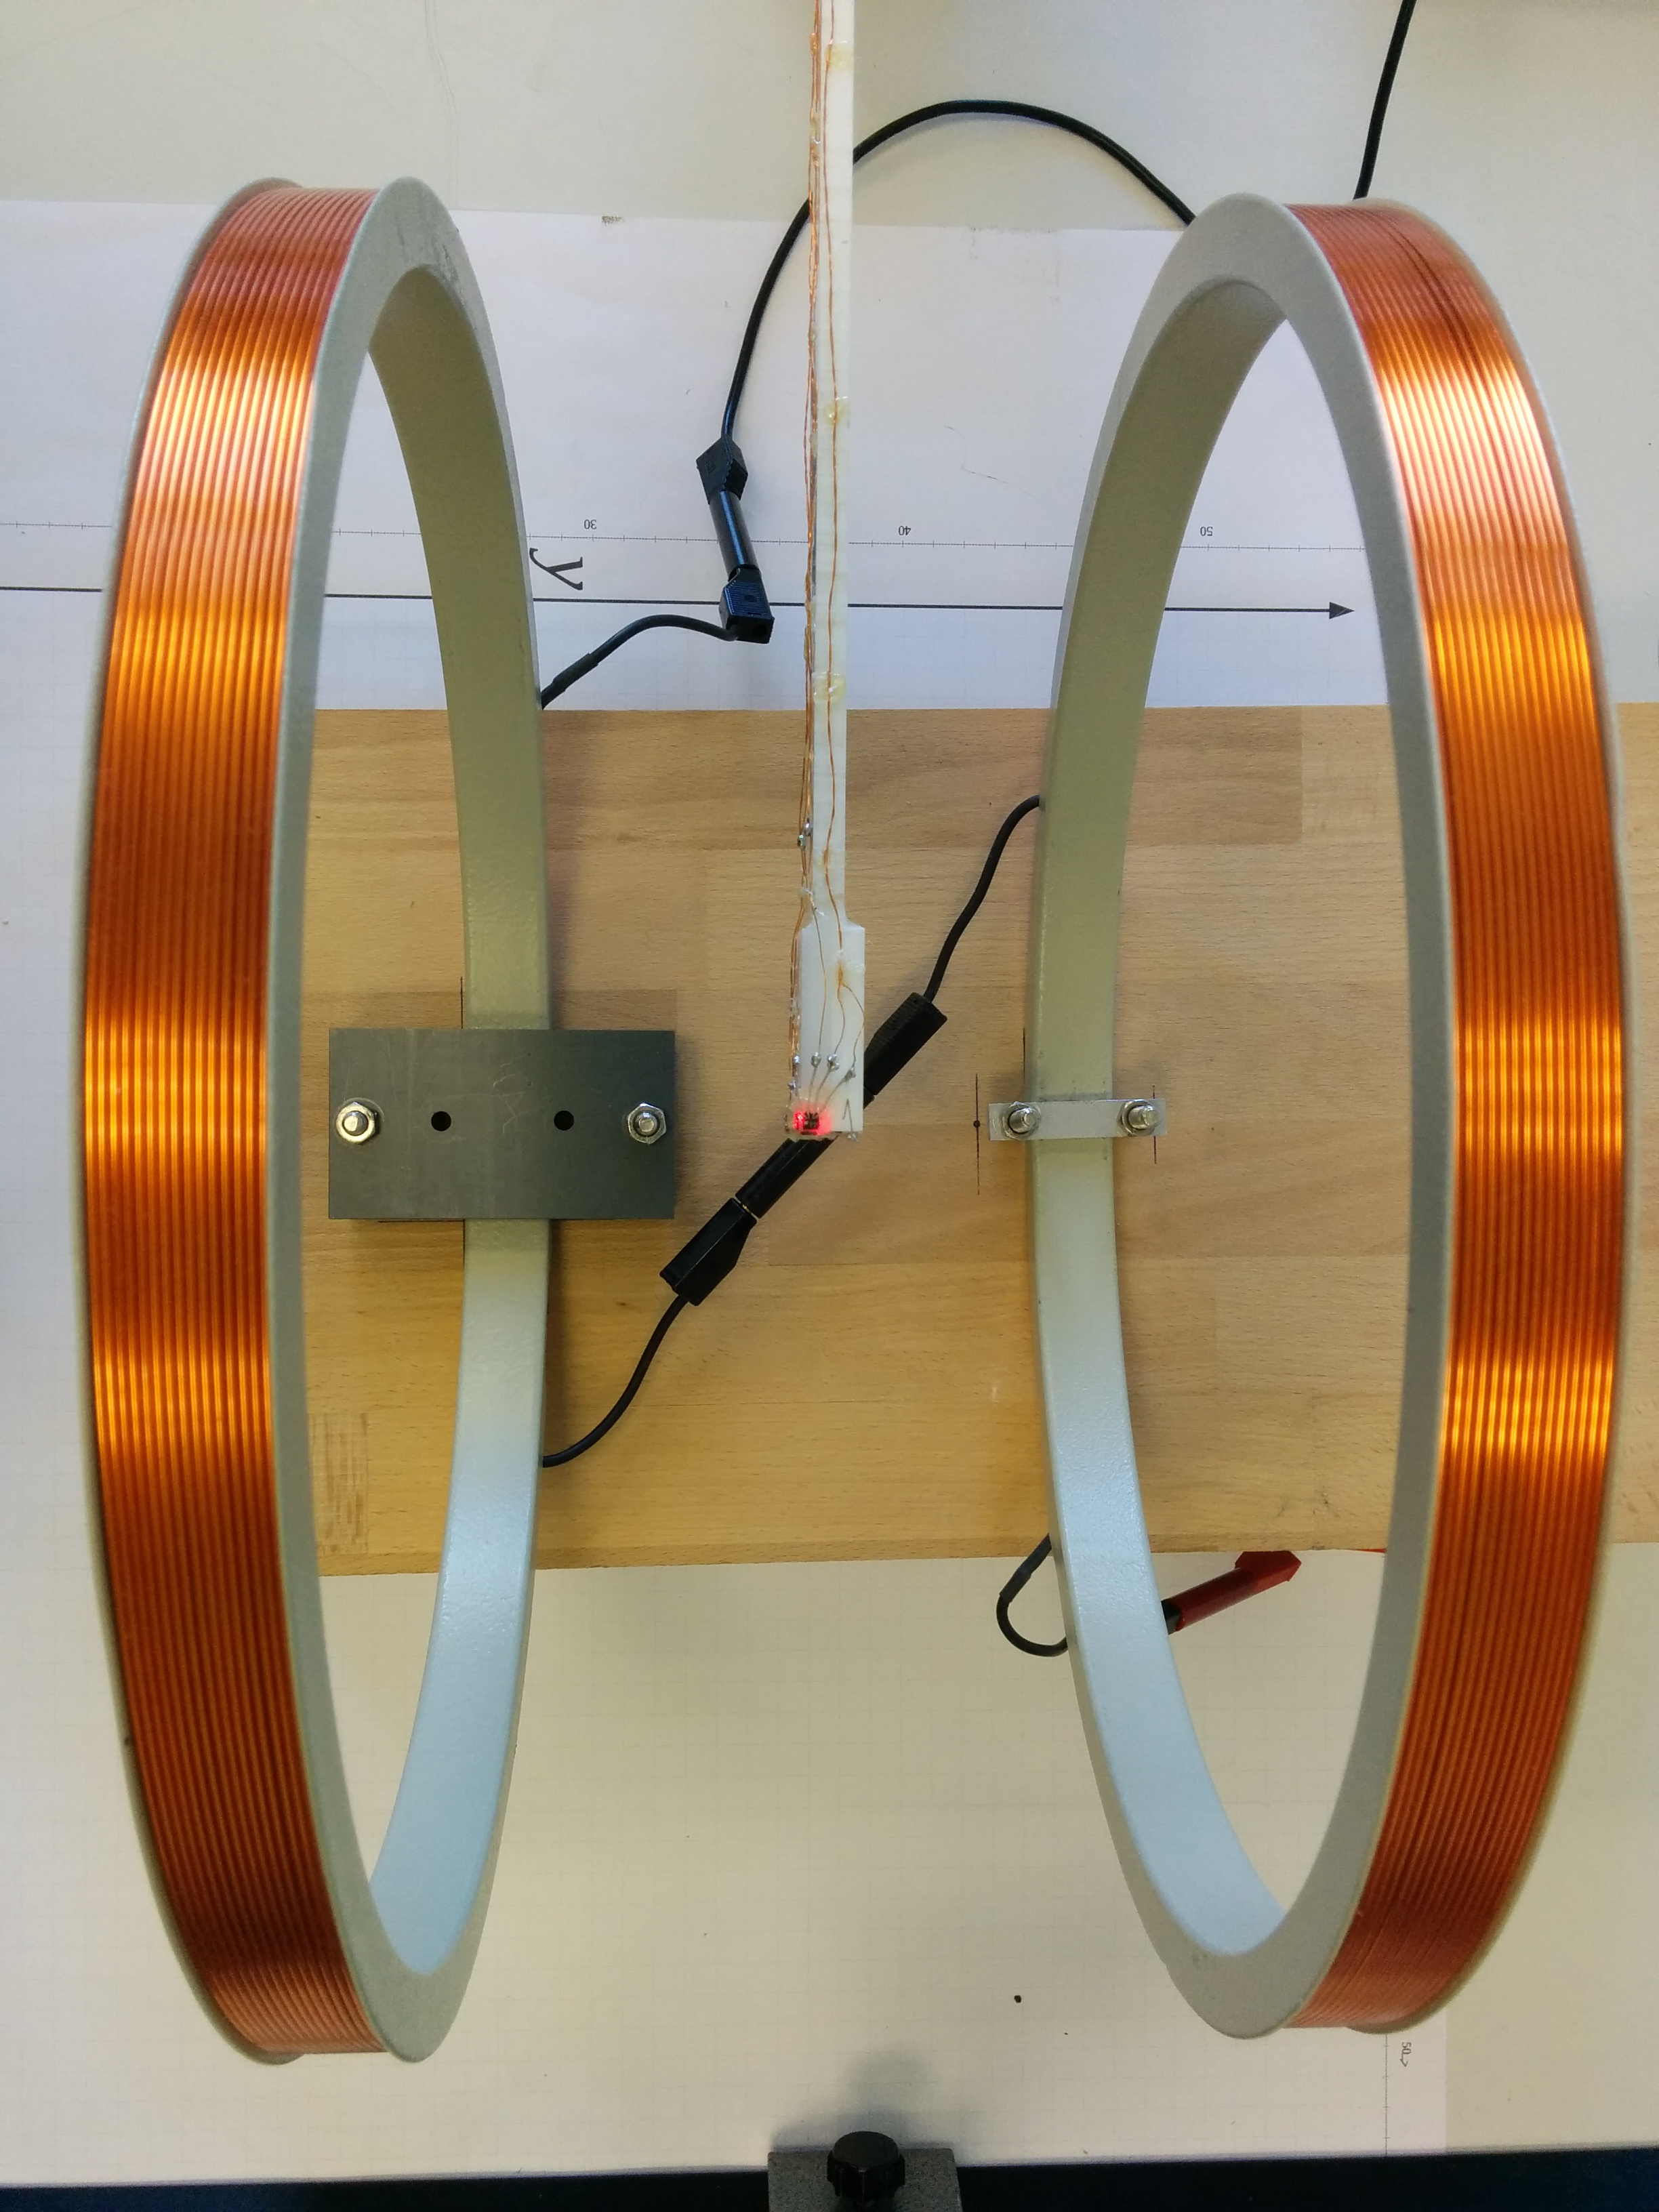
\includegraphics[scale=0.1]{durchfuehrung3.jpg}
	\caption{Ausrichtung der Sonde mittels Laser. Man erkennt den Lichtfleck an der stelle der Hallsonden und die Parallelität des Sensormaterials zur }
	\label{durchf3}
\end{figure}
\begin{figure}[H]
	\centering
	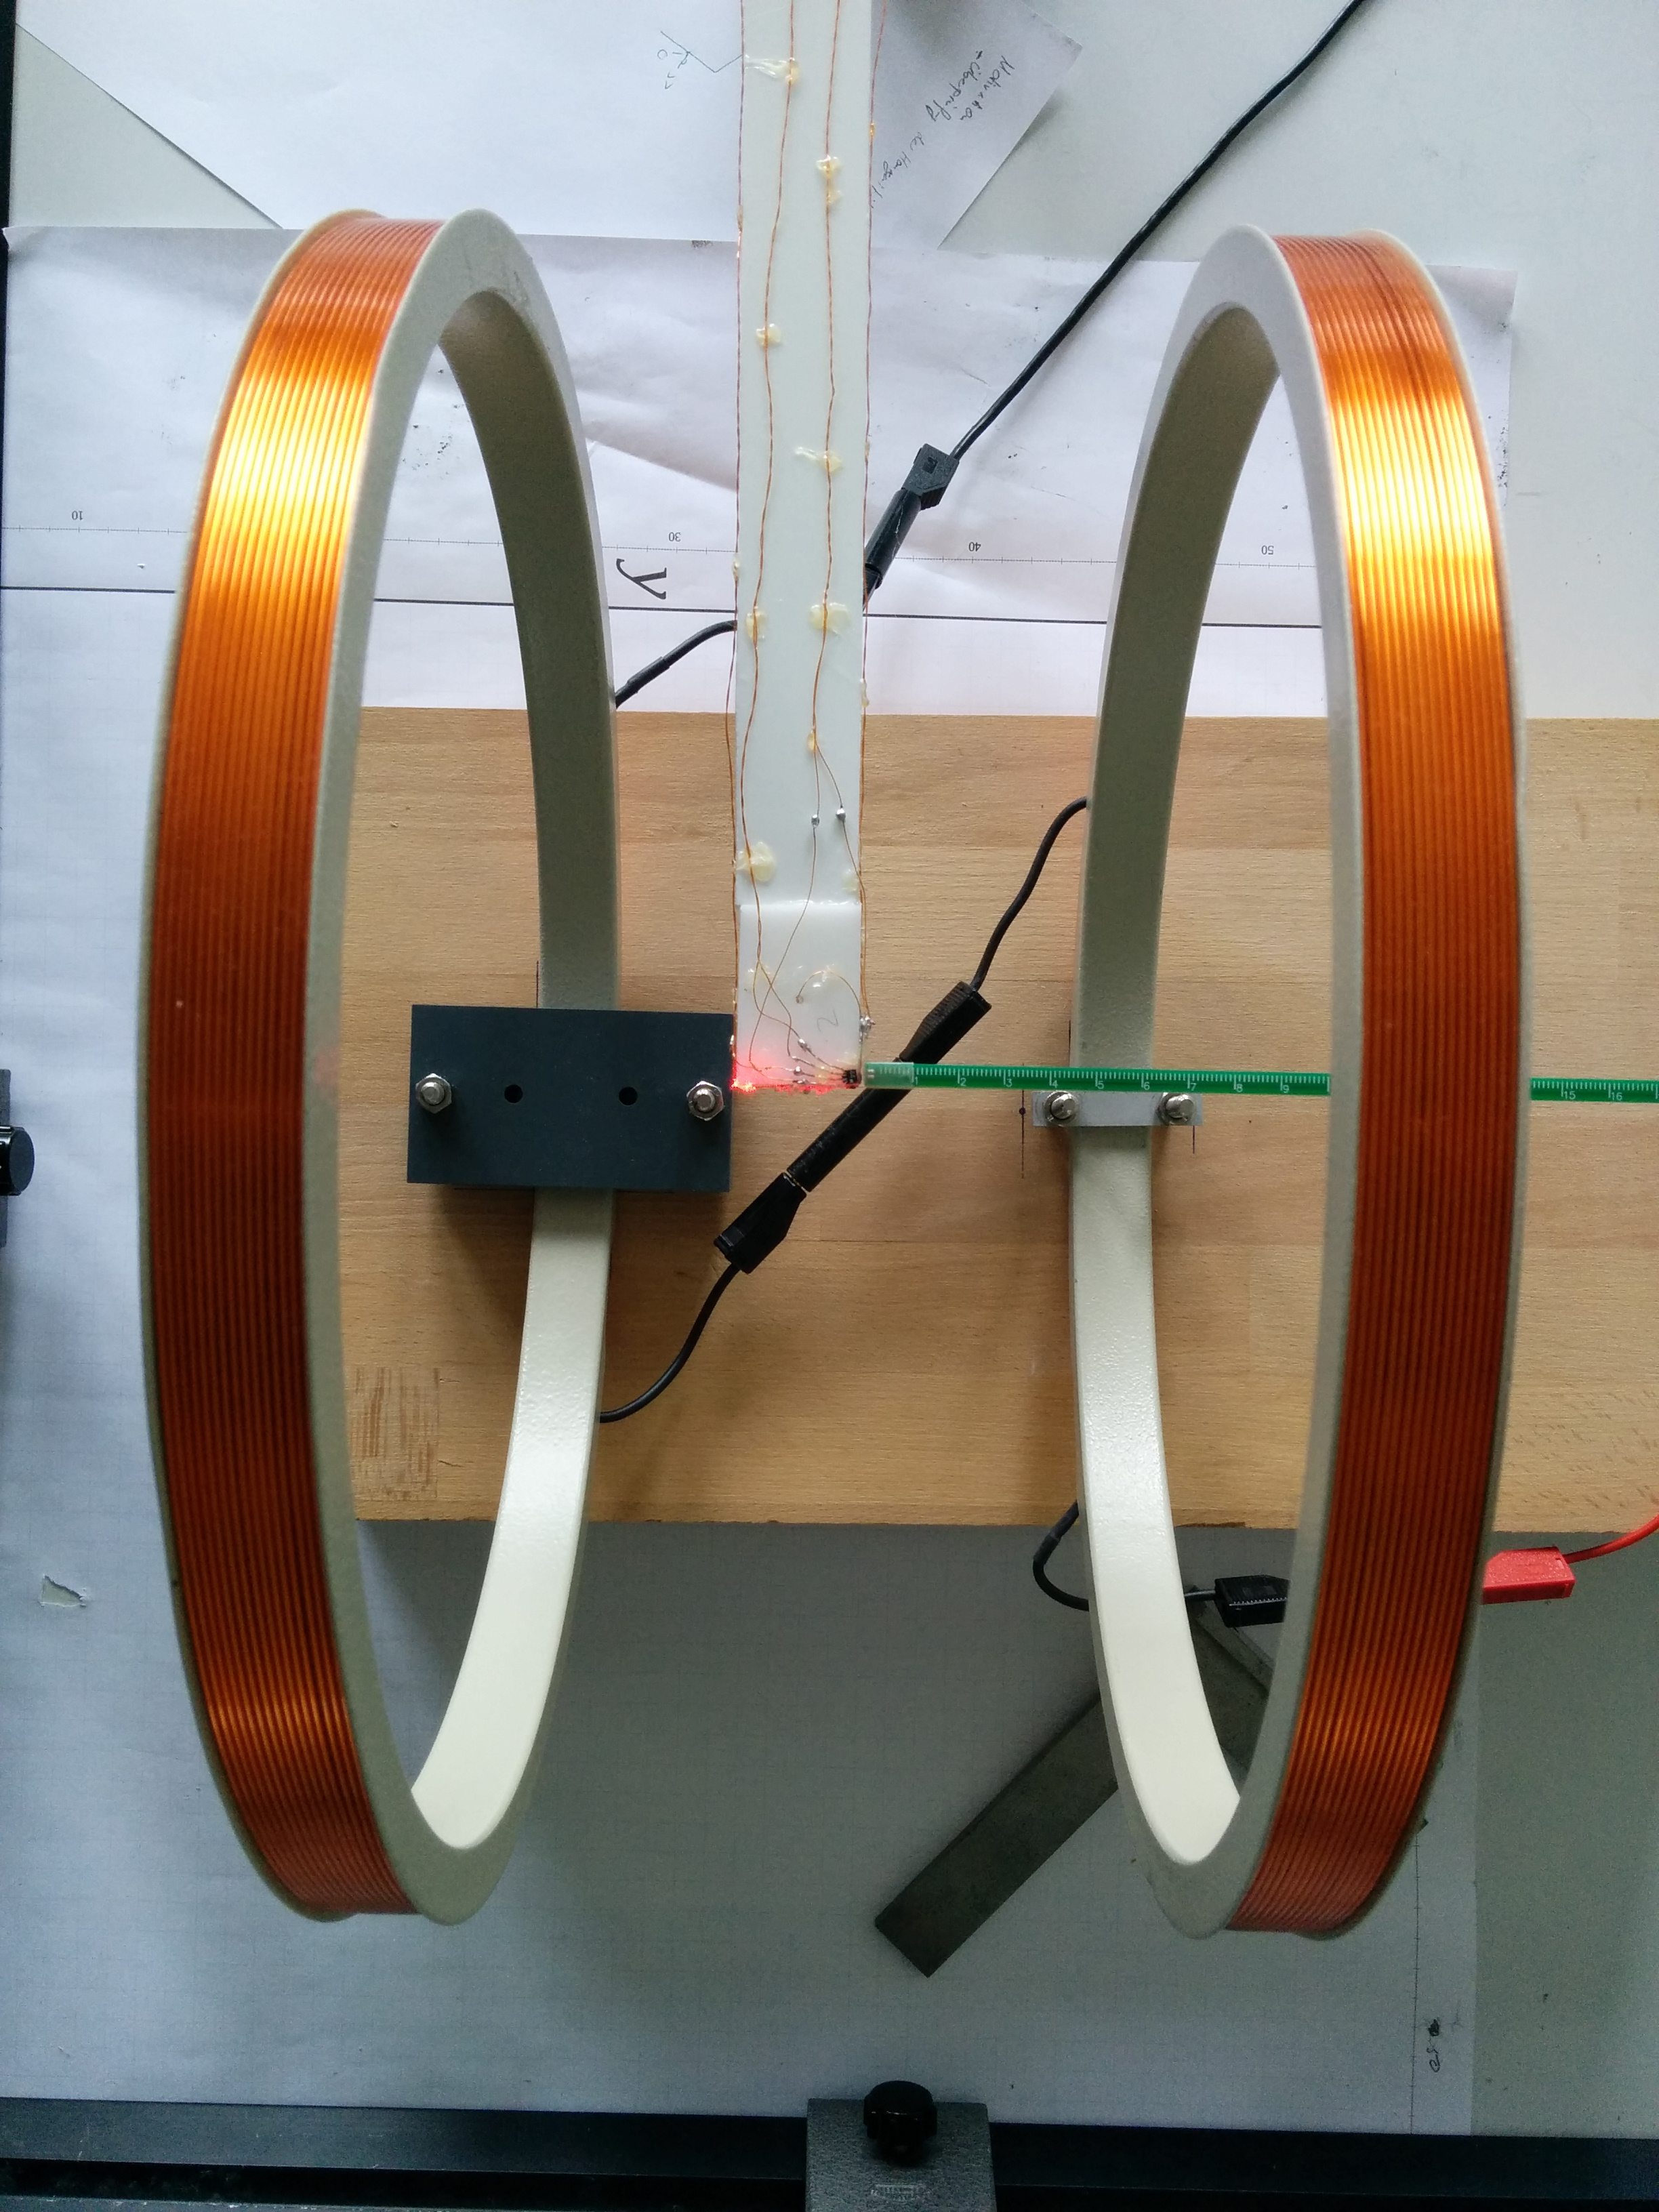
\includegraphics[scale=0.1]{kalib1.jpg}
	\caption{Fotografie des Aufbaus während der Kalibration von Sensor 1 (z-Richtung). Die Cassy-Sonde (grün) steht senkrecht zu der zu kalibrierenden Sonde. Der Messpunkt ist in der Mitte des Spulenpaars, wo das Magnetfeld aus Symmetriegründen nur in y-Richtung (hier rechts) zeigen kann.}
	\label{kalib1}
\end{figure}

\begin{figure}[H]
	\centering
	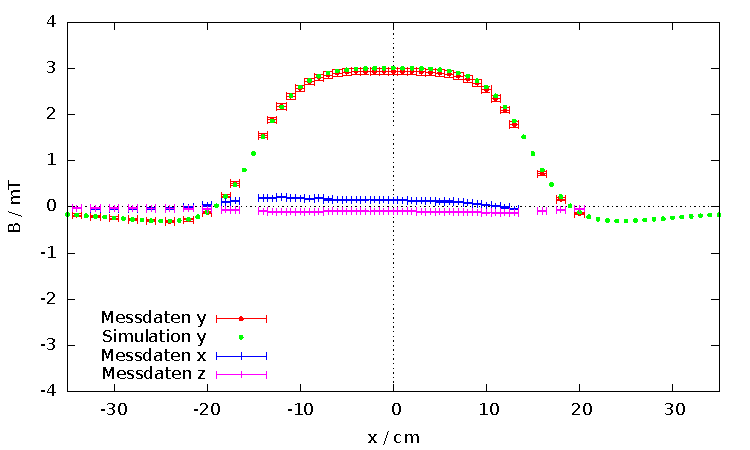
\includegraphics[scale=1]{abs1_Auswertung_parallel_2}
	\caption{Messdaten entlang der Geraden mit y=0, z=4. Die theoretische x- und z-Komponente ist konstant 0.}
	\label{fig:p2}
\end{figure}
\begin{figure}[H]
	\centering
	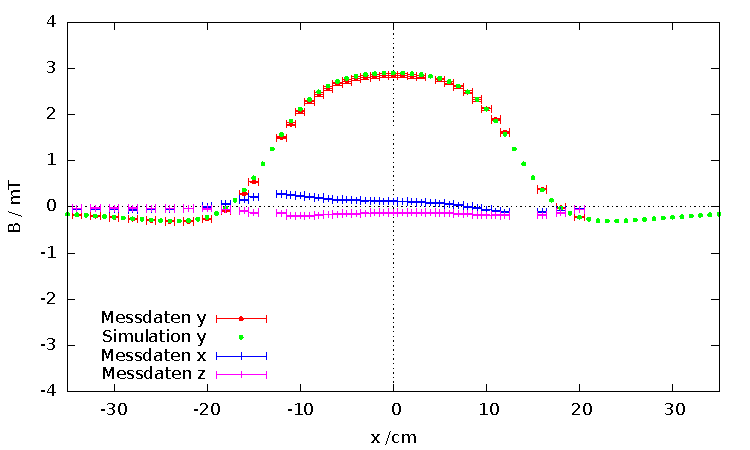
\includegraphics[scale=1]{abs1_Auswertung_parallel_3}
	\caption{Messdaten entlang der Geraden mit y=0, z=8. Die theoretische x- und z-Komponente ist konstant 0.}
	\label{fig:p3}
\end{figure}
\begin{figure}[H]
	\centering
	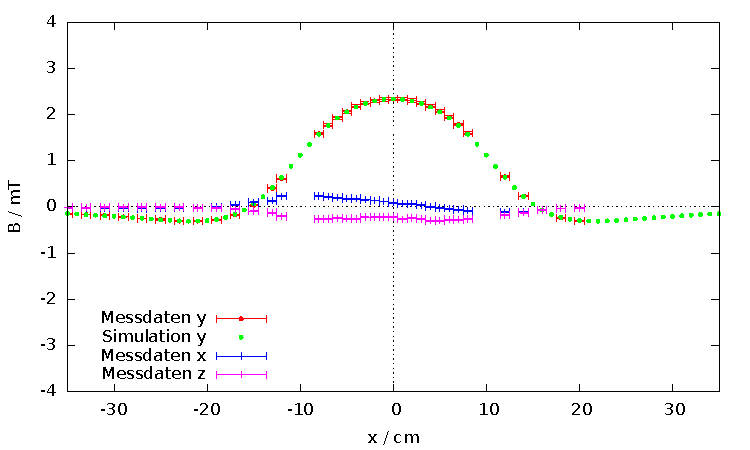
\includegraphics[scale=1]{abs1_Auswertung_parallel_4}
	\caption{Messdaten entlang der Geraden mit y=0, z=12. Die theoretische x- und z-Komponente ist konstant 0.}
	\label{fig:p4}
\end{figure}
\begin{figure}[H]
	\centering
	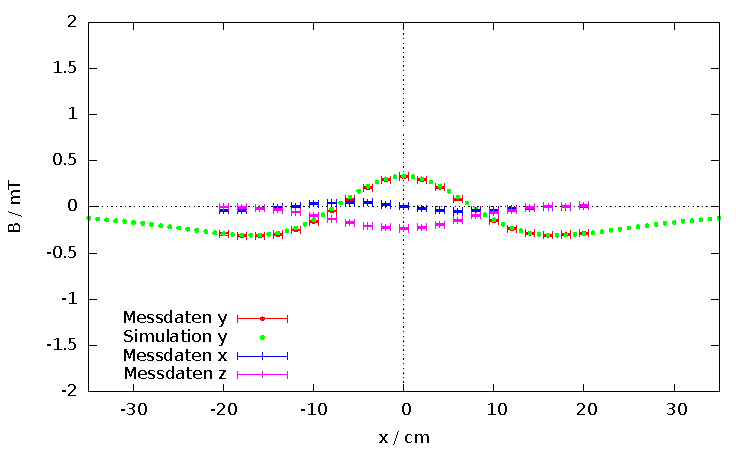
\includegraphics[scale=1]{abs1_Auswertung_parallel_5}
	\caption{Messdaten entlang der Geraden mit y=0, z=18. Die theoretische x- und z-Komponente ist konstant 0.}
	\label{fig:p5}
\end{figure}
\begin{figure}[H]
	\centering
	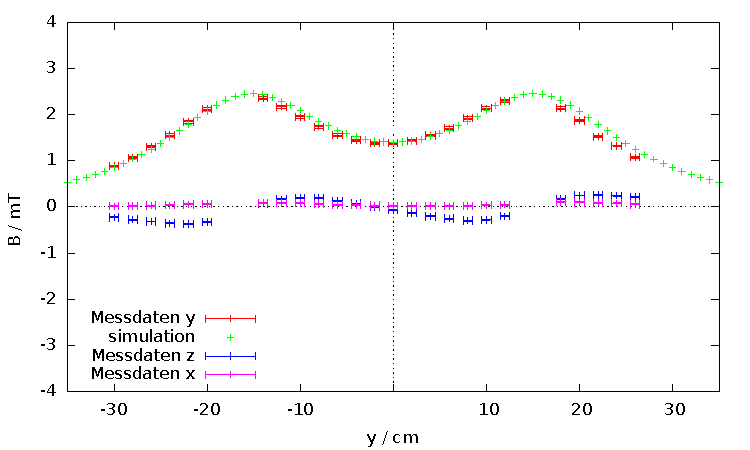
\includegraphics[scale=1]{abs2_Auswertung_axial_1.pdf}
	\caption{Messdaten mit doppeltem Spulenabstand parallel zur y-Achse mit z=5.}
	\label{fig:p6}
\end{figure}
\begin{figure}[H]
	\centering
	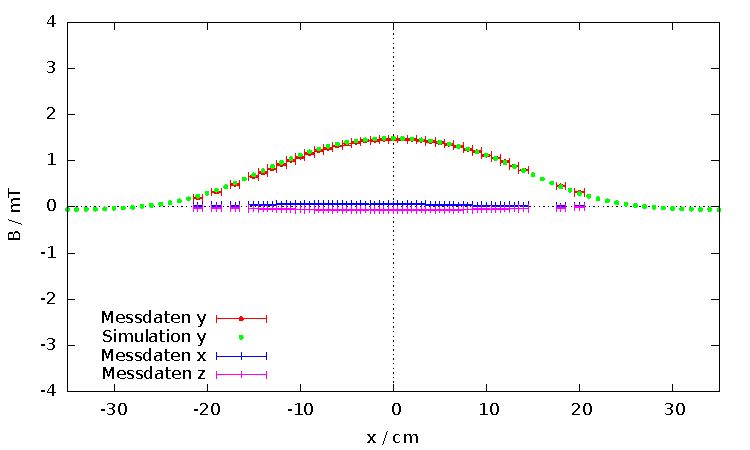
\includegraphics[scale=1]{abs21.pdf}
	\caption{Messdaten mit doppeltem Spulenabstand parallel zur x-Achse mit z=4cm.}
	\label{fig:p7}
\end{figure}
\begin{figure}[H]
	\centering
	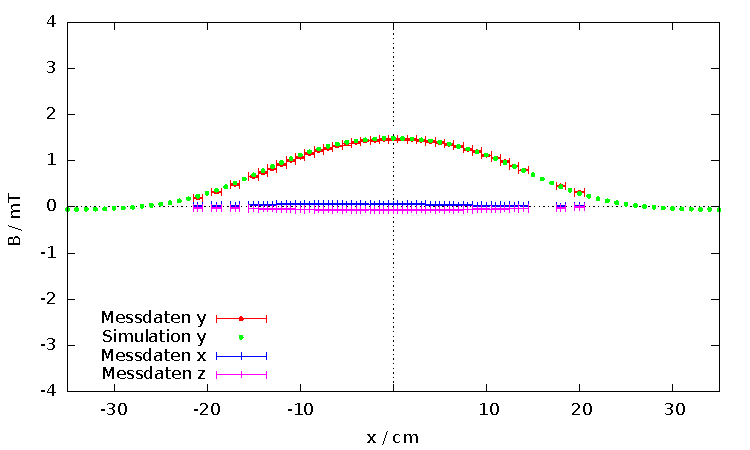
\includegraphics[scale=1]{abs22.pdf}
	\caption{Messdaten mit doppeltem Spulenabstand parallel zur x-Achse mit z=8cm.}
	\label{fig:p8}
\end{figure}
\newpage
\subsection{Zusätzliche Formeln}
\label{eq_formeln}
Für $\alpha _n$, $\beta _n$, $\gamma _n$ klein gilt:
\begin{align}
\label{eq:e1}
 \nonumber A=\frac{-sin(\alpha_3) sin(\beta_1)}{cos(\gamma_1) cos(\gamma_3)}-\frac{sin(\alpha_1) sin(\beta_2)}{cos(\gamma_1) cos(\gamma_2)}-\frac{sin(\alpha_2) sin(\beta_3)}{cos(\gamma_2) cos(\gamma_3)}\\
 +\frac{sin(\alpha_1) sin(\alpha_2) sin(\alpha_3)}{cos(\gamma_1) cos(\gamma_2) cos(\gamma_3)}+\frac{sin(\beta_1) sin(\beta_2) sin(\beta_3)}{cos(\gamma_1) cos(\gamma_2) cos(\gamma_3)}+1 \simeq 1
\end{align}
\newpage
\addcontentsline{toc}{section}{Literatur}
\bibliography{literatur}
\end{document}